%!TEX root = ../thesis.tex
%\input{commands.tex}
%*******************************************************************************
%****************************** Third Chapter **********************************
%*******************************************************************************
\chapter{Haplotype phasing consistency as a signal for physical linkage in scaffolding and assembly}

% **************************** Define Graphics Path **************************
\ifpdf
    \graphicspath{{Chapter4/Figs/Raster/}{Chapter4/Figs/PDF/}{Chapter4/Figs/}}
\else
    \graphicspath{{Chapter4/Figs/Vector/}{Chapter4/Figs/}}
\fi



\section{Background}
\par{
Reference genomes have enabled a range of genomic analysis by providing prior knowledge of the sequence 
and giving genomic context as well as a common coordinate system by which to compare multiple genomes\cite{1000genomes}\cite{GRCh38}. Assembling reference genomes is complicated by repetitive sequences, heterozygosity, and sequencing errors. As discussed in Chapter 3, when an assembly encounters inexact homologous sequences, it must determine which of these cases the sequence differences are due to. 
If the assembler cannot distinguish between heterozygosity and repeats, and if no reads span the homologous sequence into more unique regions, the contig must end
to avoid assembling distant regions or sequence from different chromosomes together. Historically reference genomes were created by sequencing and overlapping set of large haploid bacterial artificial chromosomes (BACs), yeast artificial chromosomes (YACs), and fosmid clone libraries \cite{human} (100-200kb, 100-1000kb, and 30-50kb respectively). 
These methods overcame much of the problem of resolving repeats and heterozygosity because their length allowed them to read through all but the longest segmental duplications and the fact that they are inherently haploid. However, because each of these BACs were sequenced with Sanger sequencing and assembled, they were still subject to problems in repeats longer than the Sanger reads (500bp-1kb) that were close enough to one another to occur in the same BAC clone. But most importantly, these methods are far too costly to apply to many genomes. The human genome project took 13 years to complete and cost approximately 3 billion dollars\cite{genomeproject}. Despite the labor intensive and costly process, the resulting reference genome still had errors and was not complete\cite{renamegrch38}.
} 

\par{
More recently the cost reductions of long read PacBio and Oxford Nanopore (ONT) technologies\cite{pacbio} \cite{oxford}, and improved accuracy profiles through optimization of the circular consensus method\cite{ccs}\cite{HIFI}
as well as the emergence of other long range genetic information technologies\cite{10xlinked}\cite{HiC}\cite{bionano} 
have converged to make high quality, cost effective reference genomes achievable. This has then resparked interest in assembly 
as well as large reference generation projects. Efforts have begun on the Earth Biogenome Project (EBP)\cite{EBGP}, a global project to sequence the entire diversity of multicellular eukaryotic life. In the UK, the Sanger Institute and partners have started to sequence 60,000 species from the British Isles in the Darwin Tree of Life (DToL) project. These projects aim to provide a scientific resource for the next generation of biological science, for environmental conservation, and to study evolution at a much broader and deeper scale than ever before. And for the human genome, we continue to make progress through new technologies and computational methods\cite{Wenger2019}\cite{tobias1}\cite{eichler1}. The telomere to telomere project uses multiple technologies on a cell line derived from a haploid genome from the CHM13 hydatidiform mole to create the most complete human genome to date\cite{T2T2}\cite{T2T1}.
} 

\par{
As discussed in Chapter 3, one of the primary remaining difficulties in assembling reference quality genomes is high levels of heterozygosity such as found in many of the non-model organisms included in the EBP and DToL projects. While Chapter 3 focused on going from a pool of individuals---and thus many haplotypes---to a single individual---and thus two haplotypes, this chapter focuses on the problems encountered with high levels of heterozygosity within an individual and the improvements that can be made computationally to both alleviate those problems as well as use the high levels of heterozygosity to our advantage. 
For these newer technologies mentioned above, there are now assembly algorithms that deal with each data type\cite{falcon}\cite{supernova}\cite{bionano_assembly} 
as well as combinations of multiple technologies\cite{genemyers}\cite{hybrid10x}\cite{hicscafffirst}\cite{hicassembly}. 
 These methods try to co-assemble both haplotypes arriving at a haploid consensus \cite{watchtower} \cite{canu} 
 or a diploid assembly\cite{falconphase}\cite{supernova}\cite{hifiasm}\cite{dipasm}, but heterozygosity still injects complexity and ambiguity on top of a haploid assembly process.
} 

\par{
As mentioned in Chapter 3, one method for dealing with the problem of heterozygosity is inbreeding organisms to a point of low heterozygosity \cite{drosophila}, 
but this is not possible for all organisms. Trio-sga used pedigree information in the assembly algorithm \cite{trio-sga} 
but was built exclusively for short reads. Recently Koren et al. described trio binning which uses a mother-father-child trio to 
separate long reads into their haplotype of origin prior to haploid assembly\cite{triobinning}. 
While this method is very effective, creating such a cross would be infeasible for many species and costly for the vast number of reference genomes these projects intend to sequence. 
Another recent approach using the new highly accurate High Fidelity (HiFIi) CCS reads from PacBio along with homopolymer compression and other methods to reduce errors dramatically is to 
require nearly identical sequence similarity to extend the assembly graph\cite{HICANU}. This results in the haplotypes being assembled separately in all but the few long stretches of homozygosity in 
a genome. They then run a haplotic purging software PurgeDups\cite{purgedups} to remove one of the haplotype assemblies. This has the downside of not matching the haplotypes to make comparisons, but that could be done 
fairly well as an additional analysis step. This method does not explicitly phase the haplotypes and may have long phase switch errors especially across long regions of homozygosity. DipAsm does a first pass assembly followed by haplotype phasing and separation of the reads by haplotype prior to haploid assembly\cite{Garg2021}.
} 

\par{
Despite the incredible advances made over the past several years in both sequencing technologies and assembly methods, we still cannot assemble whole chromosomes or chromosome arms with a 
single technology for most organisms. After assembly we are left with some level of fragmentation of chromosomes into contiguous sequences (contigs) which we wish to scaffold together. While the 
PacBio HiFi technology has many beneficial properties including continuous, highly accurate reads, it does not produce long enough reads to span all repeat or low sequence complexity regions in most genomes.
 10x Genomics linked read technology, however, will create barcode linked short reads across much longer molecules (50kb+) with some molecules reaching well over 250kb\cite{10xlinked}. Optical map technology in which the DNA is linearized and flourescent markers are attached to sequence specific loci via restriction digestion and optically inspected can give sparse data for pieces of DNA about as long as can be isolated with modern high molecular weight extraction methods\cite{opticalmaps1}. And high-throughput chromatin conformation capture sequencing (Hi-C) data creates links between sequences physically located close to one another. While there will be cross-chromosomal links, the large majority of links are intra-chromosomal but can create links of almost any length\cite{3CHIC}\cite{hic2}. Each of these technologies have been used both to break misassemblies in contigs and scaffold contigs\cite{scaff10x}\cite{opticalmaphuman}\cite{hicscafffirst}\cite{SALSA}\cite{GRAAL}\cite{instaGRAAL}. But some of these scaffolders have been known to introduce misassemblies\cite{hicscafffirst}. 
} 


\par{
While high levels of heterozygosity make the assembly problem harder for traditional methods, haplotype phasing consistency (the consistent separation of heterozygous alleles into distinct groups corresponding to the haplotype they belong to) can be used as a signal of physical linkage in both assembly and scaffolding and as a method to differentiate inexact repeats from haplotype differences. While the conventional thinking is that heterozygosity makes these problems more difficult, we turn this around and use the phasing consistent property of heterozygous sites as a powerful way to simplify and add statistical power to them. This is made possible by the advent of long read and other long genetic range information technologies, as short reads would not span enough distance to consistently link heterozygous sites. In this chapter I present a toolkit for phasing, phasing aware assembly, and phasing aware scaffolding called phasstools (Phasing and Assembly tools). The code is open source and available at \href{https://github.com/wheaton5/phasstools}{https://github.com/wheaton5/phasstools}. The use cases are reference based and fully de novo haplotype phasing, assembly based phasing aware scaffolding, and phasing aware assembly. While I will show results from the phasing aware assembly, these are preliminary and not without problems, which I will discuss. For that reason, I will first address the steps required to use phasing consistency for highly accurate assembly scaffolding. First I will outline phasing consistency, then introduce heterozygous single nucleotide polymorphism (SNP) kmer pairs as a mechanism for \textit{de novo} haplotype phasing. Next I introduce an algorithm for \textit{de novo} haplotype phasing using sparse \textit{Bernoulli} mixture model clustering---an algorithm very similar to the clustering algorithm used in Chapter 2. I discuss some several benefits and limitations of this algorithm for our purposes. I then move on to another phasing algorithm based on a given assembly to that can be used for phasing aware scaffolding. I show results for both phasing algorithms on a dataset from the Darwin Tree of Life program from the butterfly \textit{Vanessa atalanta}. }

\par{
Next I consider haploid sex contig detection, because these contigs will need to be treated differently in the steps going forward. Before scaffolding, I discuss breaking contigs that are incorrectly joined in a chimeric misassembly using Hi-C linkage information and the phasing consistency of those links across the midpoint of a moving window. Finally, I discuss phasing aware scaffolding and the results on \textit{Vanessa atalanta} HiCanu assembly. }

\par{
I then continue by discussing the incomplete phased assembly process. I first consider a process of using the pairwise phasing consistencies to create a phased assembly graph, but then show several error modes that this process can encounter. This lead us to need to use more than pairwise phasing consistency. I show how the system recruits each subsequent kmer pair and decide whether to add it to the graph or not and how it updates future potential kmer pair's phasing consistency counts. After this process, the assembly phase blocks are used to separate HiFi reads into haplotype bins and do haploid assemblies of each of those read bins. I show this process on the same butterfly dataset of \textit{Vanessa atalanta} and compare our assemblies to the HiCanu assembly of the same data. I show high concordance with the HiCanu assembly, but with lower contiguity as well as not assembling the haploid sex chromosomes. This work shows the power of using phasing consistency as a strong signal for physical linkage in diploid chromosomes.
}


\section{Phasing aware scaffolding of an existing assembly: phasst scaff}

\par{
Our goal is to use the phasing consistency of Hi-C reads and, optionally, linked reads that cover heterozygous sequence on two contigs. First, the heterozygous sites must be identified. Then phasing consistency of those sites can be defined.
}

\subsection{Heterozygous kmer pairs and detection}
\par{
In the case of scaffolding an existing assembly, one could map the reads to the assembly and call variants to find heterozygous sites as is the common workflow for resequencing efforts. In an effort to be unbiased by the 
assembly, and to be general to a \textit{de novo} assembly process, I tackle the subject of identifying heterozygous variants in a reference-free manner. I do this using a kmer approach, as many reference-free methods do. 
Many people have focused on identifying kmers which occur at roughly half counts in short read data\cite{KAT} and various software exists to count kmers\cite{jellyfish} 
and to model the mixture of expected distributions (errors, haploid, diploid, duplication kmers)\cite{genomescope}. Identifying heterozygous kmers in this way 
suffers from multiple problems. 1. Many of these identified as half counts will be either randomly high count error kmers or randomly low count 
homozygous kmers due to the fact that the count distributions are generally not fully separated. 2. It ends up with $K-1$ overlapping kmers for a given variant which is needlessly redundant information that will both slow down any phasing algorithm and 
likely break key independence assumptions. And 3. while it identifies heterozygous kmers, one doesn't know which kmers are alternative alleles of each other. 
I instead identify pairs of kmers which vary only in the center position which are also both roughly at half counts. These heterozgyous SNP kmers 
will be much more robust and have the benefit of knowing that one is very likely to be the alternative allele of the other. The kmer count spectrum is generated with a fast disk backed kmer counter KMC\cite{kmc}\cite{kmc2}\cite{kmc3}. Figure \ref{figure:kmc} shows an example kmer count histogram. The kmer size chosen will determine how unique these kmers are in the genome as well as how likely they are to be correct in the reads. For CLR, shorter kmers must be used because kmers of any reasonable length (15+) are unlikely to be correct. But using kmers of this length mean that many of the chosen kmers will be repeats instead of heterozygous. For this reason, I limit this project to HiFi data and use a kmer size of 31 throughout.
}

\begin{figure}[htbp!]

\caption{Kmer count spectra and heterozygous paired kmers}
\label{figure:kmc}
\begin{centering}
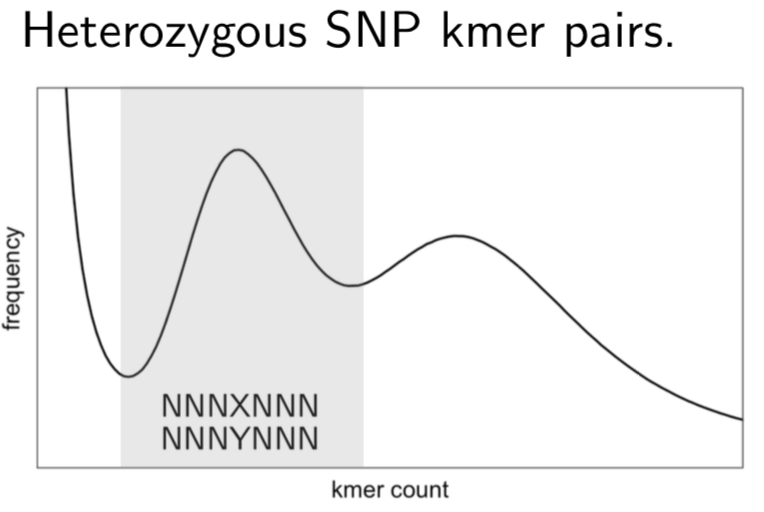
\includegraphics[width=0.65\textwidth]{kmc.png}
\par{An example of kmer count spectrum showing error kmers on the left, heterozygous kmers in the first peak and homozygous kmers in the next peak.}
\end{centering}
\end{figure}

\par{
The heterozygous range of the kmer spectra is calculated with code from purge dups\cite{purgedups}. The kmers are then dumped in alphabetical order and searched for pairs of kmers which vary in only the middle base and fall into the heterozygous counts range. A futher restriction is made that the sum of the counts of the kmers with the other two possible bases in the middle are not high. A very high repeat count may produce, through sequencing errors or mutations, two lower count kmers differing in the middle base. It should also be noted that while I generally refer to these kmer pairs as heterozygous kmer pairs, they may also represent paralogous kmer pairs. The phasing consistency of these kmer pairs with others is used to determine if they are more likely to be from heterozygous or paralogous sequences. Each produces a characteristic pattern in the pairwise kmer consistency counts.
}

\subsection{Read data kmer information}
\par{
I use the kmers in the reads to determine if heterozygous paired kmers are phasing consistent with other paired kmers. For each read of each technology (Hi-C, PacBio, linked reads) the position and ID of each paired kmer is stored on disk in a custom binary format for later use. Of note here is that the linked read technology may have multiple molecules per barcode whereas in other technologies, reads represent single physically linked molecules. Richard Durbin has developed a method to \textit{de novo} assign reads from barcodes to molecule groups using shared kmers across barcode sets to cluster reads into their molecules of origin\cite{hash10x}. In this work, I chose not to use this as it is unpublished and not extensively tested. Instead, the distance in the assembly graph or contigs (if using an existing assembly) is used to determine which reads came from which barcode. With the recommended DNA input, high molecular weight (HMW) extraction sizes, and number of partitions, the Poisson loading process results in an expected number of molecules per barcode of roughly ten. Because the total amount of DNA per partition is a small percentage of the total genome sizes we work with, the chances of a partition having molecules which arose from nearby or overlapping locations is rare. Thus one can deduce that reads from a barcode which map close to one another on a reference or assembly arose from the same HMW molecule. While this is not fully \textit{de novo}, it is highly unlikely to cause a false inference because a chimeric misassembly causing incorrect linked read molecule inference would not result in a phasing consistent signal.
}

\subsection{Phasing consistency}
\par{
For each kmer pair, I refer to one as the reference allele and one as the alternate allele arbitrarily without loss of generality. The read kmer data is used to create phasing consistency counts between different paired kmers. If the read contains the reference version of paired kmer $k_1$ and reference version of paired kmer $k_2$, the cis1 count gets incremented. We may do this with any of the data types for different purposes, but we do not combine counts across data types as the error modes are different. For example, the Hi-C data will have some spurious connections across chromosomes due to the 3D conformation of the chromosomes in a particular nucleus. For the linked reads, we may also stipulate that a version of paired kmer $k_1$ and paired kmer $k_2$ be within some distance of each other on the assembly graph or contig.
}
\subsubsection{Pairwise haplotype phasing consistency}
\par{
First the phasing consistency between pairs of kmer pairs is considered before moving on to higher order phasing consistency. With pairwise phasing consistency, there are only four potential combinations that a read can have of the two pairs (see figure \ref{figure:consistency}). With more than two kmer pairs, the number of potential combinations increases exponentially. In order to deal with that, multiple kmers pairs will be phased with respect to one another before considering their consistency with other kmer pairs or groups of phased kmer pairs, always reducing the problem to four possibilities.
}


\begin{figure}[htbp!]
\caption{Pairwise phasing consistency counts}\label{figure:consistency}
\centering
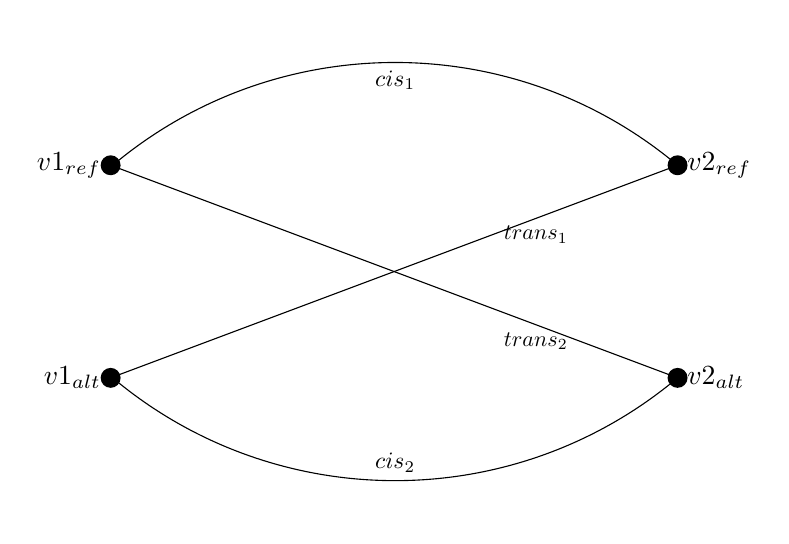
\begin{tikzpicture}[scale=1.8]
\def\xoffset{0}
\def\yoffset{0}
\def\titley{1.2}
\def\panellength{5}
\def\titlescale{1}
 \def\subtitlescale{0.7}
 \node[anchor=east] at (0 + \xoffset,2 + \yoffset) {$v1_{alt}$};
\draw (4 + \xoffset,2 + \yoffset) arc (-50:-130:3.1) node[midway,above, scale=0.85] {$cis_2$};
\fill (0 + \xoffset ,2 + \yoffset) circle[radius=2pt];
\node[anchor=west] at (4 + \xoffset,2 + \yoffset) {$v2_{alt}$};
\fill (4 + \xoffset,2 + \yoffset) circle[radius=2pt];
\node[anchor=east] at (0 + \xoffset,3.5 + \yoffset) {$v1_{ref}$};
\fill (0 + \xoffset,3.5 + \yoffset) circle[radius=2pt];
\draw (4 + \xoffset,3.5 + \yoffset) arc (50:130:3.1) node[midway,below, scale=0.85]{$cis_1$};
\draw (4 + \xoffset ,3.5 + \yoffset) -- node[below, scale=0.8] {$trans_1$} (2 + \xoffset,2.75 + \yoffset) -- (0+ \xoffset,2 + \yoffset);
\draw (4 + \xoffset,2 + \yoffset) -- node[below, scale=0.8] {$trans_2$} (2+ \xoffset,2.75 + \yoffset) -- (0+ \xoffset,3.5 + \yoffset);
\node[anchor=west] at (4+ \xoffset,3.5 + \yoffset) {$v2_{ref}$};
\fill (4+ \xoffset,3.5 + \yoffset) circle[radius=2pt];
\end{tikzpicture}
\floatfoot{\small{I denote one of each kmer pair as the reference or alternative arbitrarily. Molecules that have the sequences of one of the kmers from each of two kmer pairs will fall into one of four cases represented here by the four edges in this graph. The molecules falling into each of these four categories are tabulated. Phasing consistent heterozygous kmer pairs will have counts predominantly on both cis edges or both trans edges.
}}
\end{figure}

\subsubsection{Phasing consistency and error modes}

\par{
There are several distinctive signals from pairwise phasing consistency counts and further insight can be gained when looking at those manifestations across the multiple paired kmers to which a given paired kmer is linked.
} 

\begin{figure}[htbp!]
\caption{Pairwise phasing consistency counts}\label{figure:consistency2}
\centering
\sidesubfloat[]{
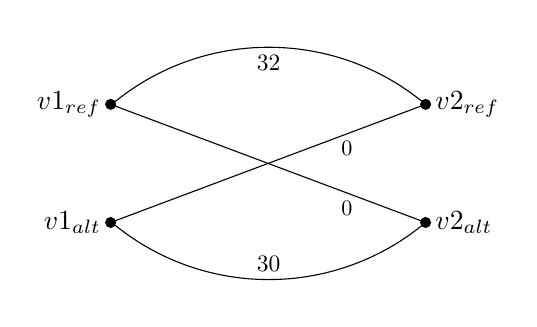
\begin{tikzpicture}[scale=1]
\def\xoffset{0}
\def\yoffset{0}

\def\titley{1.2}
\def\panellength{5}
\def\titlescale{1}
 \def\subtitlescale{0.7}
% \node[scale=\titlescale,align=center] at (0.5*\panellength+\xoffset,\titley+\yoffset){\textbf{a}. Phasing consistent in cis};

 \node[anchor=east] at (0 + \xoffset,2 + \yoffset) {$v1_{alt}$};
\draw (4 + \xoffset,2 + \yoffset) arc (-50:-130:3.1) node[midway,above, scale=0.85] {$30$};
\fill (0 + \xoffset ,2 + \yoffset) circle[radius=2pt];
\node[anchor=west] at (4 + \xoffset,2 + \yoffset) {$v2_{alt}$};
\fill (4 + \xoffset,2 + \yoffset) circle[radius=2pt];
\node[anchor=east] at (0 + \xoffset,3.5 + \yoffset) {$v1_{ref}$};
\fill (0 + \xoffset,3.5 + \yoffset) circle[radius=2pt];
\draw (4 + \xoffset,3.5 + \yoffset) arc (50:130:3.1) node[midway,below, scale=0.85]{$32$};
\draw (4 + \xoffset ,3.5 + \yoffset) -- node[below, scale=0.8] {$0$} (2 + \xoffset,2.75 + \yoffset) -- (0+ \xoffset,2 + \yoffset);
\draw (4 + \xoffset,2 + \yoffset) -- node[below, scale=0.8] {$0$} (2+ \xoffset,2.75 + \yoffset) -- (0+ \xoffset,3.5 + \yoffset);
\node[anchor=west] at (4+ \xoffset,3.5 + \yoffset) {$v2_{ref}$};
\fill (4+ \xoffset,3.5 + \yoffset) circle[radius=2pt];

\end{tikzpicture}\label{fig:a}}
\sidesubfloat[]{
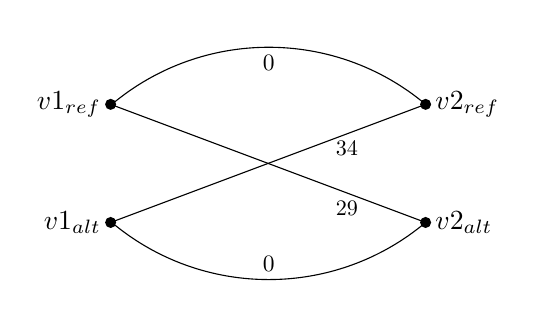
\begin{tikzpicture}[scale=1]
\def\xoffset{0}
\def\yoffset{0}

\def\titley{1.2}
\def\panellength{5}
\def\titlescale{1}
 \def\subtitlescale{0.7}
% \node[scale=\titlescale,align=center] at (0.5*\panellength+\xoffset,\titley+\yoffset){\textbf{a}. Phasing consistent in cis};

 \node[anchor=east] at (0 + \xoffset,2 + \yoffset) {$v1_{alt}$};
\draw (4 + \xoffset,2 + \yoffset) arc (-50:-130:3.1) node[midway,above, scale=0.85] {$0$};
\fill (0 + \xoffset ,2 + \yoffset) circle[radius=2pt];
\node[anchor=west] at (4 + \xoffset,2 + \yoffset) {$v2_{alt}$};
\fill (4 + \xoffset,2 + \yoffset) circle[radius=2pt];
\node[anchor=east] at (0 + \xoffset,3.5 + \yoffset) {$v1_{ref}$};
\fill (0 + \xoffset,3.5 + \yoffset) circle[radius=2pt];
\draw (4 + \xoffset,3.5 + \yoffset) arc (50:130:3.1) node[midway,below, scale=0.85]{$0$};
\draw (4 + \xoffset ,3.5 + \yoffset) -- node[below, scale=0.8] {$34$} (2 + \xoffset,2.75 + \yoffset) -- (0+ \xoffset,2 + \yoffset);
\draw (4 + \xoffset,2 + \yoffset) -- node[below, scale=0.8] {$29$} (2+ \xoffset,2.75 + \yoffset) -- (0+ \xoffset,3.5 + \yoffset);
\node[anchor=west] at (4+ \xoffset,3.5 + \yoffset) {$v2_{ref}$};
\fill (4+ \xoffset,3.5 + \yoffset) circle[radius=2pt];

\end{tikzpicture}\label{fig:b}
} \\

\sidesubfloat[]{
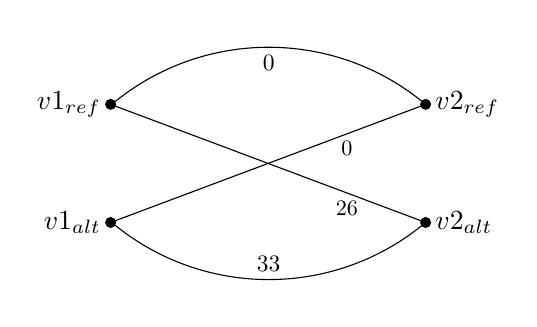
\begin{tikzpicture}[scale=1]
\def\xoffset{0}
\def\yoffset{0}

\def\titley{1.2}
\def\panellength{5}
\def\titlescale{1}
 \def\subtitlescale{0.7}
% \node[scale=\titlescale,align=center] at (0.5*\panellength+\xoffset,\titley+\yoffset){\textbf{a}. Phasing consistent in cis};

 \node[anchor=east] at (0 + \xoffset,2 + \yoffset) {$v1_{alt}$};
\draw (4 + \xoffset,2 + \yoffset) arc (-50:-130:3.1) node[midway,above, scale=0.85] {$33$};
\fill (0 + \xoffset ,2 + \yoffset) circle[radius=2pt];
\node[anchor=west] at (4 + \xoffset,2 + \yoffset) {$v2_{alt}$};
\fill (4 + \xoffset,2 + \yoffset) circle[radius=2pt];
\node[anchor=east] at (0 + \xoffset,3.5 + \yoffset) {$v1_{ref}$};
\fill (0 + \xoffset,3.5 + \yoffset) circle[radius=2pt];
\draw (4 + \xoffset,3.5 + \yoffset) arc (50:130:3.1) node[midway,below, scale=0.85]{$0$};
\draw (4 + \xoffset ,3.5 + \yoffset) -- node[below, scale=0.8] {$0$} (2 + \xoffset,2.75 + \yoffset) -- (0+ \xoffset,2 + \yoffset);
\draw (4 + \xoffset,2 + \yoffset) -- node[below, scale=0.8] {$26$} (2+ \xoffset,2.75 + \yoffset) -- (0+ \xoffset,3.5 + \yoffset);
\node[anchor=west] at (4+ \xoffset,3.5 + \yoffset) {$v2_{ref}$};
\fill (4+ \xoffset,3.5 + \yoffset) circle[radius=2pt];

\end{tikzpicture}\label{fig:c}}
\sidesubfloat[]{
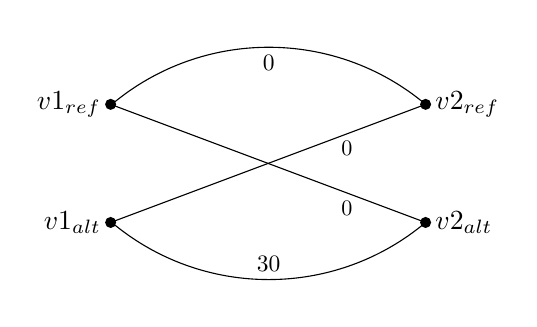
\begin{tikzpicture}[scale=1]
\def\xoffset{0}
\def\yoffset{0}

\def\titley{1.2}
\def\panellength{5}
\def\titlescale{1}
 \def\subtitlescale{0.7}
% \node[scale=\titlescale,align=center] at (0.5*\panellength+\xoffset,\titley+\yoffset){\textbf{a}. Phasing consistent in cis};

 \node[anchor=east] at (0 + \xoffset,2 + \yoffset) {$v1_{alt}$};
\draw (4 + \xoffset,2 + \yoffset) arc (-50:-130:3.1) node[midway,above, scale=0.85] {$30$};
\fill (0 + \xoffset ,2 + \yoffset) circle[radius=2pt];
\node[anchor=west] at (4 + \xoffset,2 + \yoffset) {$v2_{alt}$};
\fill (4 + \xoffset,2 + \yoffset) circle[radius=2pt];
\node[anchor=east] at (0 + \xoffset,3.5 + \yoffset) {$v1_{ref}$};
\fill (0 + \xoffset,3.5 + \yoffset) circle[radius=2pt];
\draw (4 + \xoffset,3.5 + \yoffset) arc (50:130:3.1) node[midway,below, scale=0.85]{$0$};
\draw (4 + \xoffset ,3.5 + \yoffset) -- node[below, scale=0.8] {$0$} (2 + \xoffset,2.75 + \yoffset) -- (0+ \xoffset,2 + \yoffset);
\draw (4 + \xoffset,2 + \yoffset) -- node[below, scale=0.8] {$0$} (2+ \xoffset,2.75 + \yoffset) -- (0+ \xoffset,3.5 + \yoffset);
\node[anchor=west] at (4+ \xoffset,3.5 + \yoffset) {$v2_{ref}$};
\fill (4+ \xoffset,3.5 + \yoffset) circle[radius=2pt];

\end{tikzpicture}\label{fig:d}
}

\floatfoot{\small{Example of a phasing consistent pair of heterozygous paired kmers \textbf{a)} in cis and \textbf{b)} in trans. \textbf{c)} shows an example of phasing inconsistency because the v2 kmer pair are not a heterozygous kmer pair, but because of paralogous sequence. The reference version of the v2 pair probably exists elsewhere in the genome. If this were due to a tandem repeat, we might expect all four edges to contain counts, perhaps with two edges having fewer counts due to fewer reads reaching into the 2nd repeat. \textbf{d)} shows a somewhat ambiguous case. From this, we do not know if v1 or v2 is heterozygous or not. This could arise from both being homozygous or one of them being heterozygous, but its pair not being the other haplotype.
}}
\end{figure}

\par{
Figure \ref{figure:consistency2} shows the main phasing consistent and inconsistent phenotypes for pairs of paired kmers. It is uncommon to get very mixed signals especially when working with HiFi data. When working with Hi-C data, pairwise counts are not of much use as it is rare for many Hi-C read pairs to link the same two heterozygous kmer pairs. Due to ambiguous cases that should be expected from data outlined in figure \ref{figure:consistency2}d), it is not always possible to categorize kmer pairs as heterozygous or paralogous from phasing consistency counts with one other kmer pair. The phasing consistency counts that a single kmer pair has with all of the kmer pairs with which it shares enough counts can be used to find some kmer pairs that are phasing consistent with some others and inconsistent with another set due to those other kmer pairs arising from paralogous sequence. Another set of kmer pairs are inconsistent with nearly all other kmer pairs because they were not truly heterozygous.
}



\subsection{Multiple heterozygous site haplotype phasing consistency}

\par{
When using phasing consistency as a signal for assembly scaffolding, all heterozygous kmer pairs in one contig are compared to all heterozygous kmer pairs in another contig. Figure \ref{figure:scaff} outlines what that looks like in the same way the previous phasing consistency diagrams did for pairs of individual kmer pairs. In order to do this, the heterozygous kmer pairs within each contig must be phased with respect to each other.
}

\begin{figure}[htbp!]
\caption{Phasing aware scaffolding}
\label{figure:scaff}
\begin{centering}
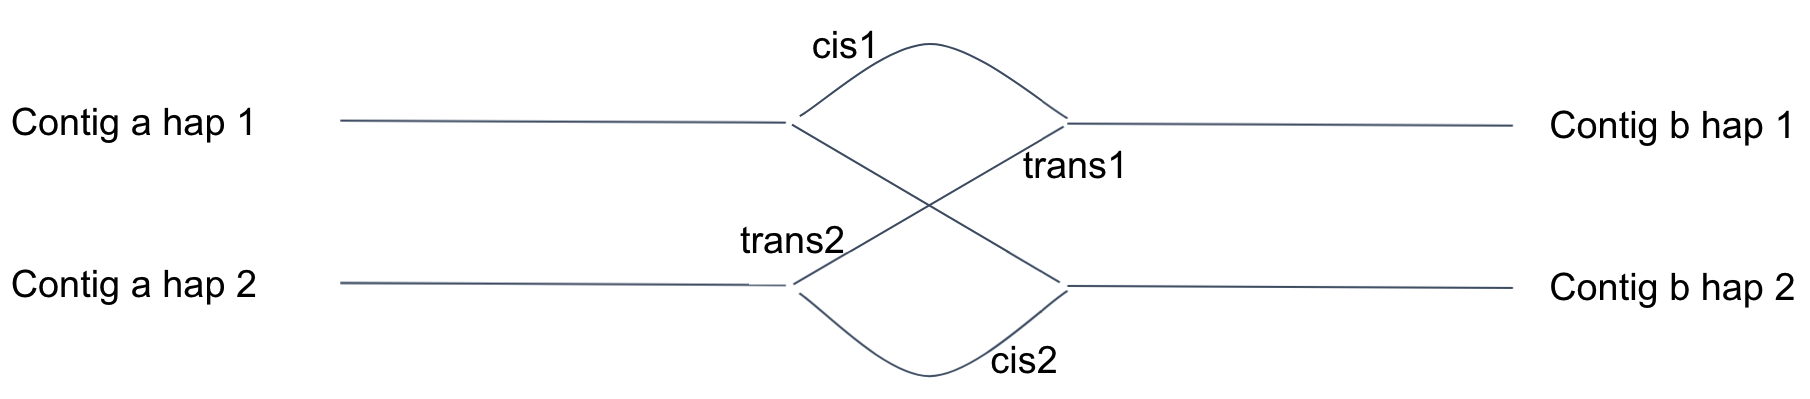
\includegraphics[width=\textwidth]{phasescaff.png}
\floatfoot{\small{Using phasing consistency for scaffolding requires all of the heterozygous kmer pairs within a contig to already be phased with respect to one another.}}
\end{centering}
\end{figure}



\subsection{\textit{de novo} haplotype phasing}

\par{
A combination of data types are used to \textit{de novo} haplotype phase. The data type that is required is Hi-C, but long reads or linked reads can be used in addition to them. The reason Hi-C data is required is due to the very long range genetic information it gives us. With Hi-C, it is possible to phase whole chromosomes instead of potentially having to break the phasing into phase blocks that are smaller than the chromosome. While there are existing phasing algorithms that can take multiple data types including Hi-C\cite{hapcut2}\cite{HICphasing}, I have developed my own phasing algorithm that has several benefits in general and meets our specific purposes. In addition to phasing in a \textit{de novo} fashion, this algorithm is robust to non heterozygous sequence inputs (which our kmer pairs will have) and can correct these genotypes. It also has the added benefit of being trivially extendable to polyploid genomes.
}

\subsubsection{Sparse \textit{Bernoulli} mixture model clustering}

\par{
I treat the haplotype phasing problem as a clustering problem. We first consider the diploid case. By clustering reads according to heterozygous kmer pair alleles they contain, this gives an implicit phasing of each kmer pair. Similar to the clustering algorithm in Chapter 2, I treat the haplotype clusters as vectors of allele fractions. Where in Chapter 2 this represented the probability parameter of a binomial because the underlying data were allele counts, here it will represent the probability parameter of a \textit{Bernoulli} as I make the assumption that a single read can only have one or the other of two alternate alleles. Of course each haplotype will only have one allele, but treating it as a continuous number instead of a discrete number opens the door to continuous numerical optimization methods which are often faster than discrete combinatorial optimization techniques. The optimization process then can drive the allele fraction numbers to 0 or 1 if the data supports that outcome. \\
} 

\begin{figure}[htbp!]
\caption{Sparse \textit{Bernoulli} mixture model clustering haplotype phasing}
\label{figure:scaff}
\begin{centering}
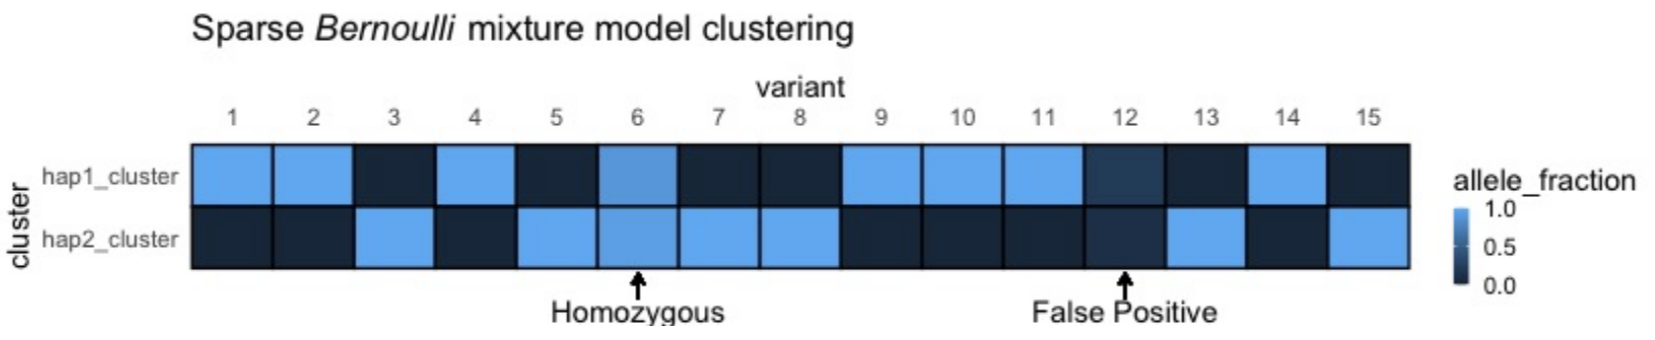
\includegraphics[width=\textwidth]{sparsebernoulli.png}
\floatfoot{\small{The phasing problem is treated as a sparse clustering problem in which reads are clustered into haplotypes.}}
\end{centering}
\end{figure}

\textbf{Definitions:}
\begin{itemize}
\item $H$: number of haplotypes. Lower case h will be used for indexing and referring to a specific haplotype.
\item $R$: number of reads. Lower case r will be used for indexing and referring to a specific read. 
\item $V$: number of kmer pairs. Lower case $v$ will be used to index and refer to a specific locus. $V_r$ will be a list of kmer pairs with observed data in read $r$.
\item $A$: Alleles. $A_{v,r}$ is a boolean representing whether read $r$ for kmer pair $v$ had the alternative allele or the reference allele.
\item $\phi_{h,v}$: cluster center value representing allele fractions of haplotype $h$ at locus $v$. The expectation is for this to be near 1.0 or 0.0 because each haplotype can only have one allele or the other, but I allow the value to be continuous to allow for continuous numerical optimization techniques and errors.
\end{itemize}

\noindent
\subsubsection{Model}

A maximum likelihood strategy is used by optimizing $\mathcal{L}(data)$ under a given model. 
\begin{equation}
\argmax_{\phi} \mathcal{L}(data, \phi)
\end{equation}


The likelihood of the data is defined by treating reads independently and marginalizing each read across the haplotypes it could belong to. 

Cluster model Likelihood function

\begin{equation}
\mathcal{L}(A) = \prod_{r \in R} \sum_{h \in H} \frac{1}{H} \prod_{v \in V_r} \begin{cases}       \phi_{h,v} & A_{v,r} == true \\      1 - \phi_{h,v} & A_{v,r} == false \\
\end{cases}
\end{equation}

\par{
This likelihood is then optimized by expectation maximization, randomly initializing cluster centers $\phi \in (0,1)$. The reader may note that due to the local nature of long reads and linked reads as well as the majority of Hi-C reads, this method can get stuck in local maxima in which for one region, the random initialization favored reads from one haplotype going to haplotype cluster 1 and in another region, reads from that same haplotype preferring haplotype cluster 2. In this case, the optimization would come into conflict at the boundary between these two regions. One could make this solve localized to a window and grow that window over time, but this would require knowledge of the assembly and make the method not truly \textit{de novo}. Or we could build our own graph and recruit new kmer pairs as we go. Another option is to use the very long scale Hi-C links for an initial solve, thus giving the haplotype cluster centers a rough global initial solution before adding in all of the data and fine tuning the local solutions. This also requires knowledge of the assembly making it not fully \textit{de novo}, but this is what I currently do. It is also possible that employing the same deterministic annealing strategy we did in Chapter 2, it may be able to get through these local maxima, but I have not tried this.
}
\subsubsection{Polyploid phasing}
\par{
This algorithm has several advantages compared to other haplotype phasing methods. While most methods' time complexity scales super linearly, oftentimes exponentially, with ploidy, if they are able to solve polyploid phasing problems at all. In this method, since haplotypes are just cluster centers, one just adds more cluster centers to match the ploidy. It would be untrue to say that this definitely scales linearly for an optimal solution. This algorithm does not guarantee optimality but neither do most modern phasing algorithms. The only modern phasing algorithm I know of which guarantees optimality is WhatsHap, a method which uses dynamic programming to ensure optimality but does not handle gapped data such as linked reads and Hi-C well\cite{whatshap}. So while this algorithm is not optimal, and its iterations to convergence may change with ploidy, the computation per expectation maximization step scales linearly with ploidy.
}
\subsubsection{Genotype correction via phasing}

\par{
Additionally our algorithm is highly robust to being given non heterozygous sites. Most phasing algorithms assume as input a set of heterozygous variants. However, even with standard resequencing, read mapping, and variant calling, some called variants will be false positives (also known as homozygous reference) or falsely called heterozygous when they are actually homozygous for the alternative allele. They could also be heterozygous or homozygous, but not with the stated alleles. This algorithm has the valuable property that the inputs are not assumed to all be heterozygous. If they are not, the haplotype centers should be driven to the correct genotype by the data. If the reads support that this kmer pair is a false variant, the values will be driven to 0 for both haplotypes, and if the reads support the alternative on both haplotypes, the values will be both driven to 1. This type of genotype correction via phasing has been done before, but with a 3rd discrete categorical state on top of the two normal states representing a 0|1 vs 1|0 phasing\cite{mypatent}. In that method, the 3rd state represented either 0|0 or 1|1 by marginalizing across both. If that state was chosen, the posterior for each case was calculated and genotype reassigned accordingly. This does work, but has the dramatic downside of increasing the total solution space from $2^n$ to $3^n$.
} 


\begin{figure}[htbp!]
\caption{Sparse \textit{Bernoulli} mixture model phasing allows for polyploid phasing and genotype correction}
\label{figure:bernoulli}
\begin{centering}
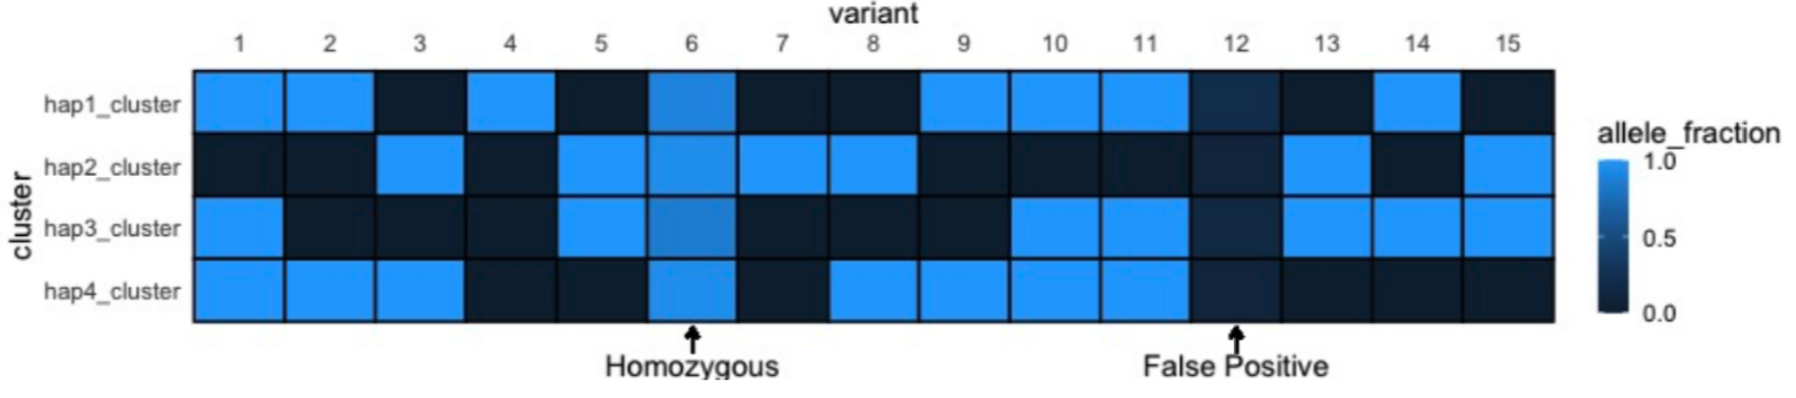
\includegraphics[width=\textwidth]{poly.png}
\floatfoot{\small{In order to handle polyploid phasing, one simply increases the number of cluster centers. And because sites are not assumed to be heterozygous, the algorithm can naturally correct miscalled genotypes.}}
\end{centering}
\end{figure}


\par{
I ran this algorithm on Hi-C, linked read, and HiFi data from a lepidoptera \textit{Vanessa atalanta} from the Darwin Tree of Life project. I then compared this phasing to which allele the HiCanu assembly 
contained. Initially I show the phasing cluster center values on a single contig to compare phasing with Hi-C alone vs with linked reads and/or long reads (see figure \ref{figure:hicphasing1}).
}

\begin{figure}[htbp!]

\caption{Phasing with Hi-C alone vs combined data}\label{figure:hicphasing1}
\begin{centering}
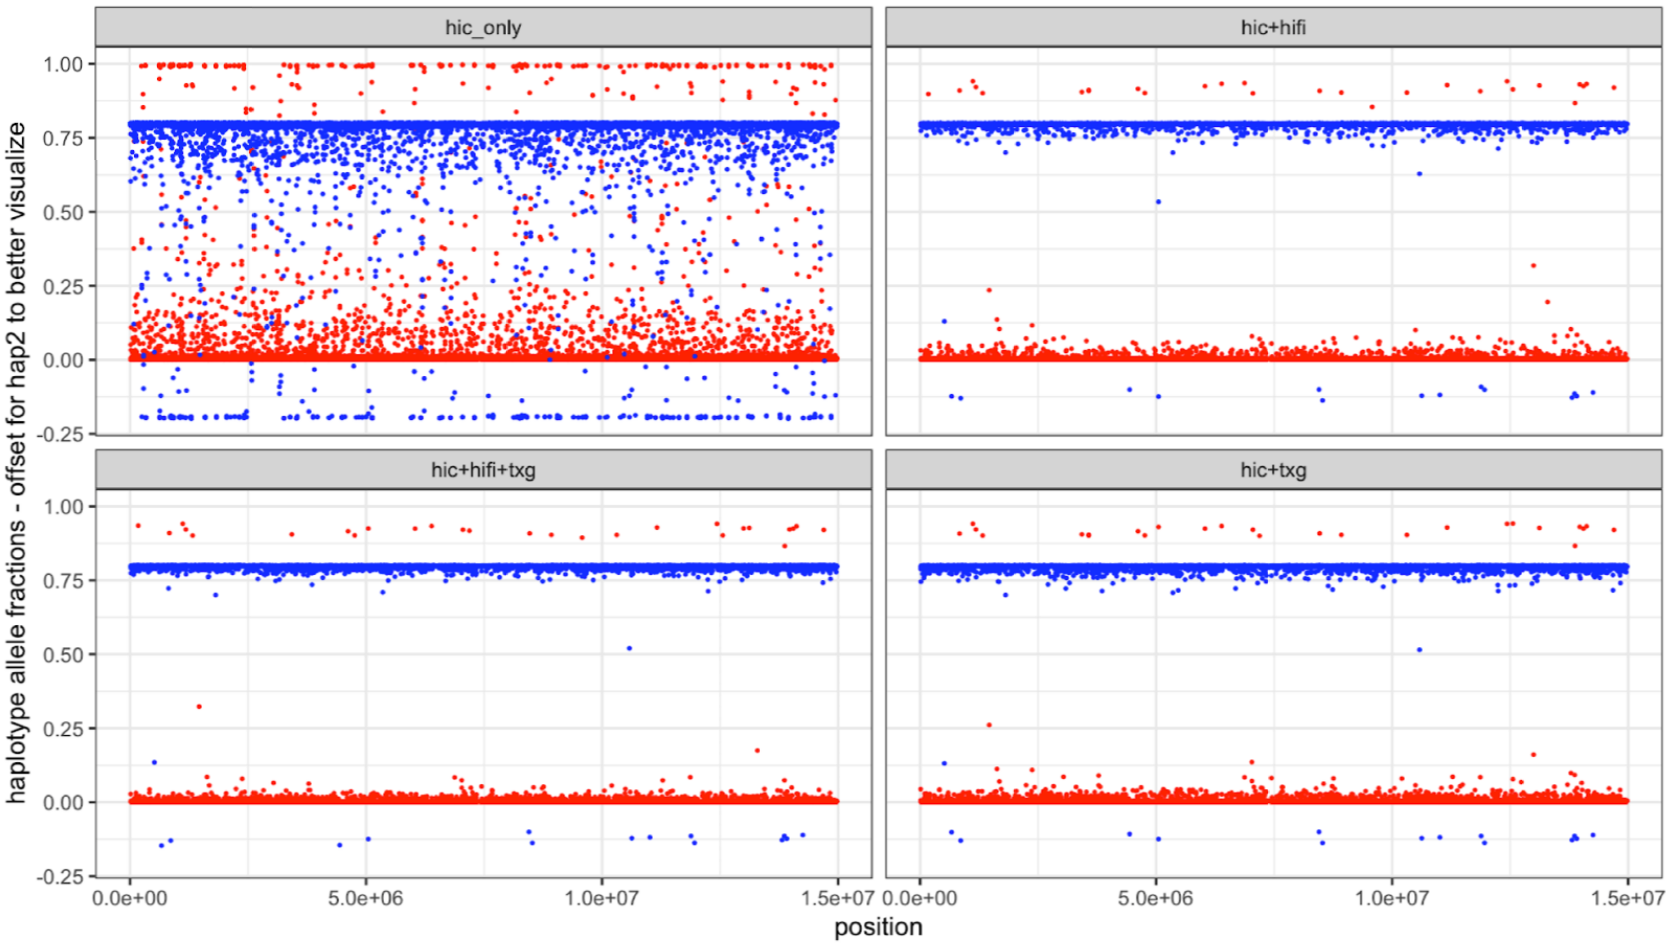
\includegraphics[width=\textwidth]{hicphasing1.png}
\floatfoot{\small{Here I show the haplotype cluster center values for sparse \textit{Bernoulli} mixture model haplotype clustering with the values for the haplotype 2 cluster offset by -0.2 such that any phase switches would be visible and not overwritten by other data points. Hi-C alone produces fairly noisy phasing probably because the chances that a HI-C read hits two heterozygous loci is fairly low reducing the total amount of useful data. When linked reads and/or HiFi reads are added, the phasing becomes much robust. *txg = 10x genomics linked reads}}
\end{centering}
\end{figure}


\par{And in figure \ref{figure:hicphasing2} I show the phasing against the entire genome.

\begin{figure}[htbp!]

\caption{Phasing \textit{Vanessa atalanta} genome}
\label{figure:hicphasing2}
\begin{centering}
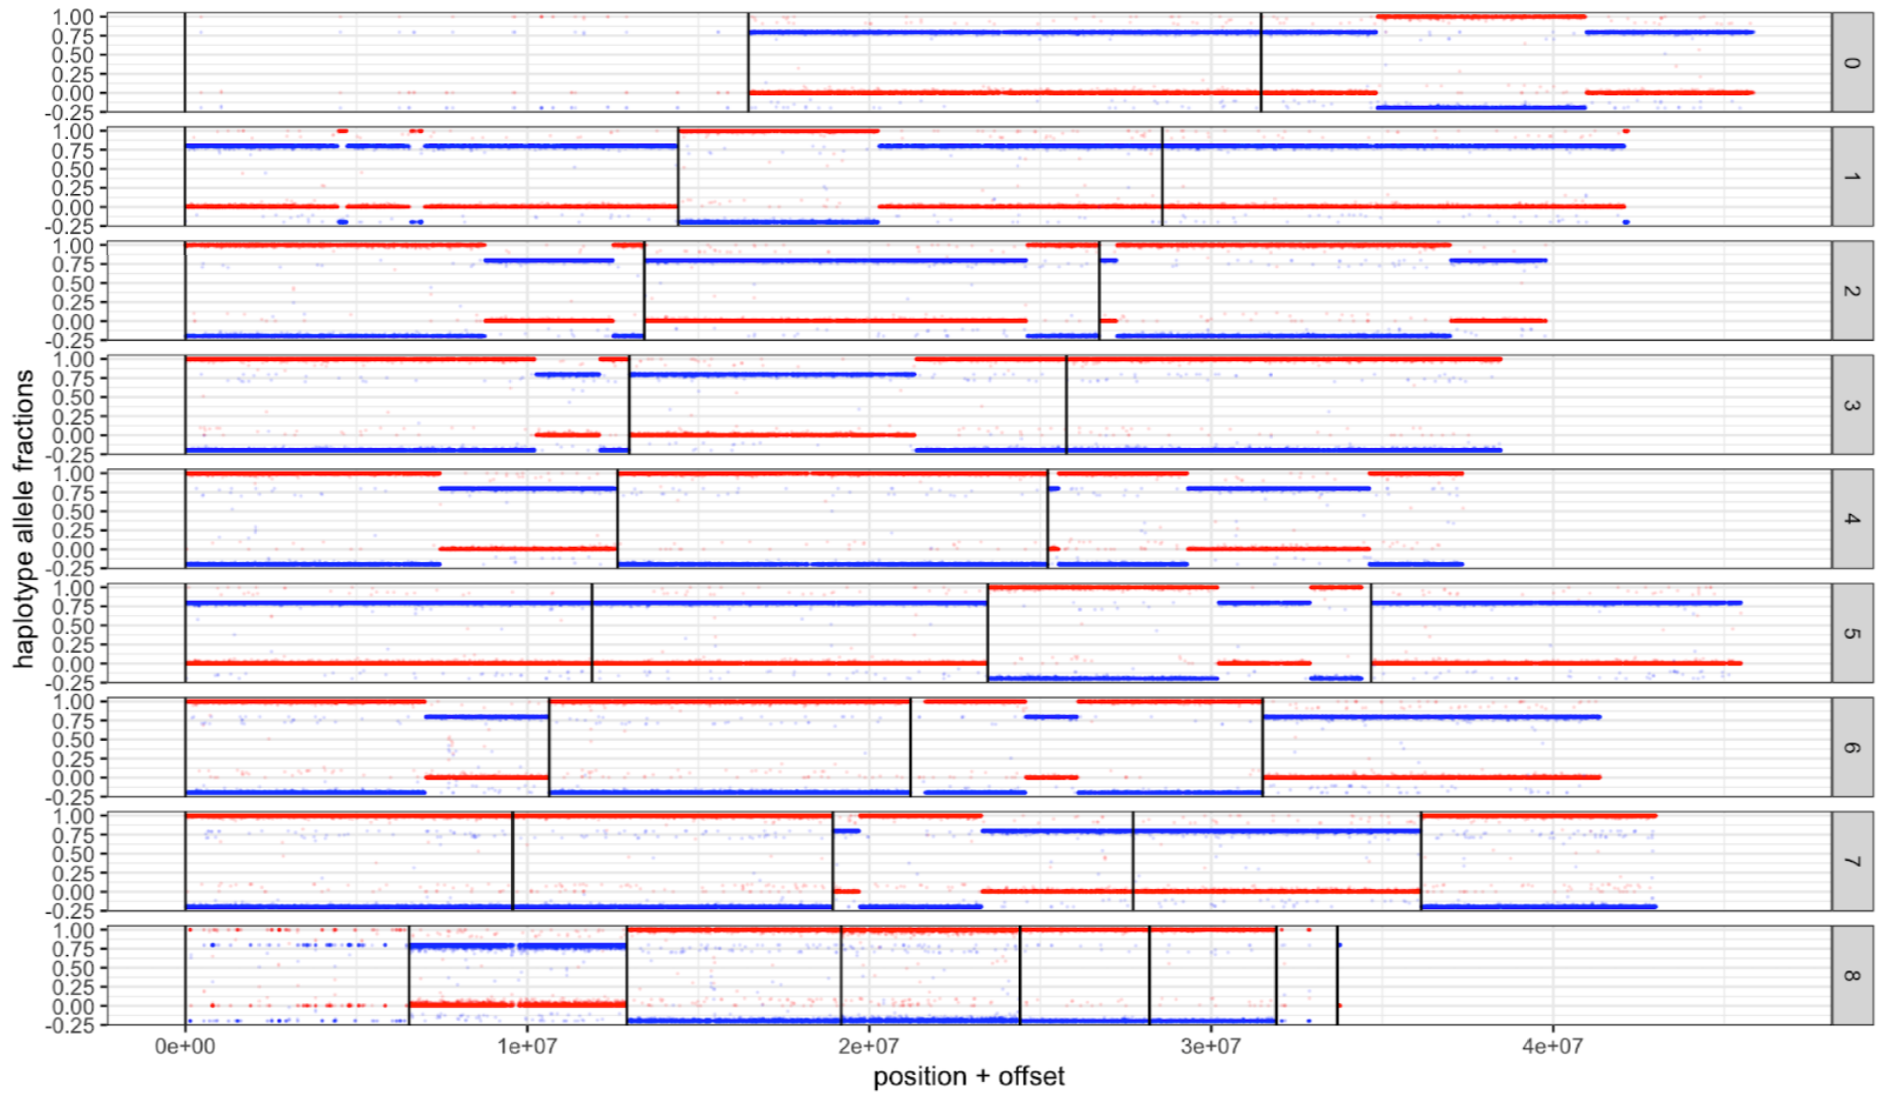
\includegraphics[width=\textwidth]{hicphasing2.png}
\floatfoot{\small{Phasing for \textit{Vanessa atalanta} genome. Here one can see that contig 1 as well as the first and last large contigs on the last row are from sex chromosomes and thus haploid. Again, the cluster center values for haplotype cluster 2 were offset down by 0.2 for visibility. And contigs are split across multiple rows for visibility. There are rare, but notable long switch errors vs the HiCanu assembly. Because my algorithm uses Hi-C data with chromosome length scale information, it is highly likely that these phase switch errors are errors in the assembly and not my phasing algorithm. }}
\end{centering}
\end{figure}

\subsection{Phasst phase: Reference or assembly based phasing}

\par{
Because the sparse \textit{Bernoulli} mixture model haplotype phasing can run into local optima, it currently requires plentiful and high quality Hi-C data. Also, for some organisms, such as diptera, chromosome pairs colocate within the nucleus\cite{somaticpairing}, greatly increasing the number of cross haplotype Hi-C links. This makes it not always sufficient to have an initial solve with just the long range Hi-C. I still believe that this algorithm can be made to work either with a moving or expanding window or through deterministic annealing, but we decided to take another direction for the time being. So I developed a reference/assembly based phasing consistency rules based phasing algorithm. First a good seed kmer is found by looking at all pairwise phasing consistencies. The kmer must have sufficient other kmers that it is phasing consistent with. Then phasing consistency counts are added for all molecules that contain this seed kmer pair to a growing data structure and mark those molecules as used. I then proceed according to the order that kmers from the paired kmer pair set occur on the assembly. If the kmer pair's phasing consistency counts are sufficient (>90\% consistent---mostly cis or mostly trans, the minor edge of the major phase---cis or trans---makes up >15\% of the counts, and the total phasing counts is at least 10), it is added to the growing phase block in the appropriate phase. Then for all molecules that contain that kmer and are not already marked used, the potential new kmer counts are updated and mark that molecule as used. This is done until the end of the contig is reached or there are a string of 10 kmer pairs with zero phasing consistency counts. I then go back to the seed kmer and proceed in the same way in the other direction.
}

\begin{figure}[htbp!]
\caption{Building phase blocks}
\label{figure:phaseblocks}
\begin{centering}
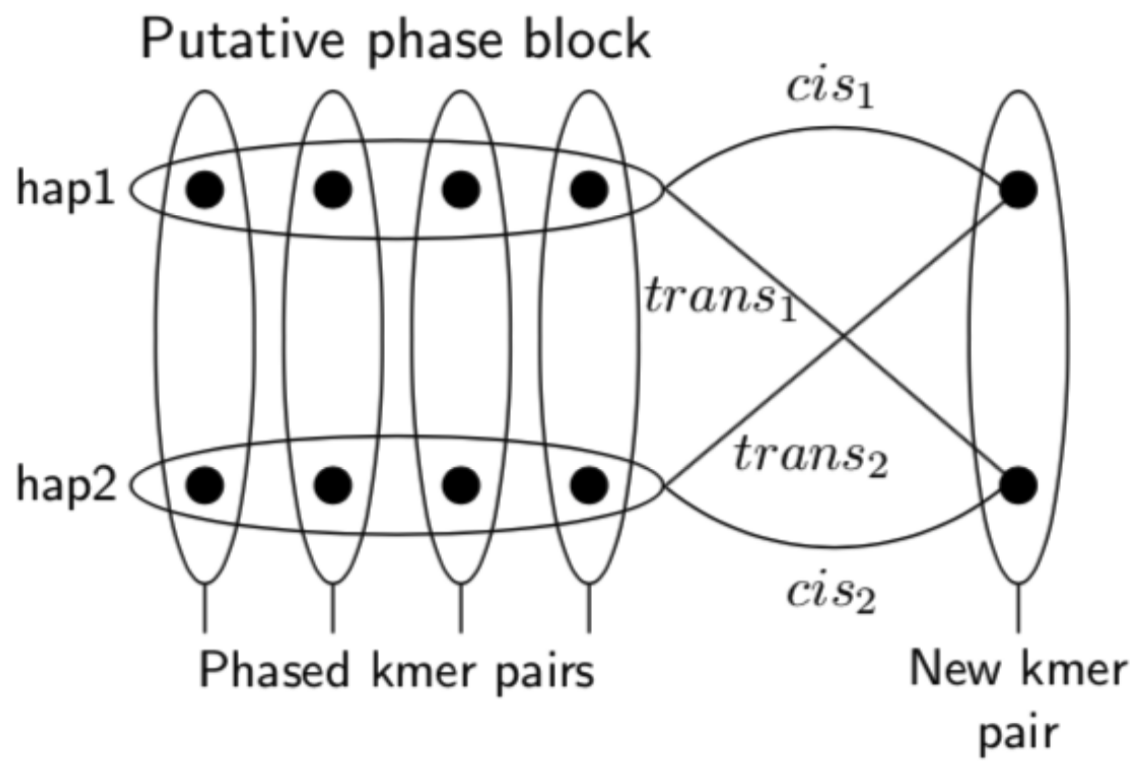
\includegraphics[width=0.6\textwidth]{phaseblockbuilding.png}
\floatfoot{{Diagram outlining the process of building phase blocks with HiFi and linked reads using phasing consistency rules. }}
\end{centering}
\end{figure}

\par{
Because only HiFi and linked reads have been used in the process thus far, it is not expected to create contig or chromosome length phase blocks. Instead, very high quality phase blocks are made that  can then be phased with respect to one another using the Hi-C reads. This is done in a way that is very similar to how Hi-C is used for phasing aware scaffolding. The Hi-C reads that have two or more phased kmer pairs in different phase blocks are used to create inter-phaseblock phasing consistency counts. Because the phase blocks are typically hundreds of kilobases long, there are plenty of Hi-C molecules linking them with two or more heterozygous kmer pairs.
} 

\par{
I ran this on the same data, this time using the HiCanu assembly post purge dups but pre-scaffolding and curation.
}


\begin{figure}[htbp!]
\caption{Phasst phase results on \textit{Vanessa atalanta}}
\label{figure:phasstphase}
\begin{centering}
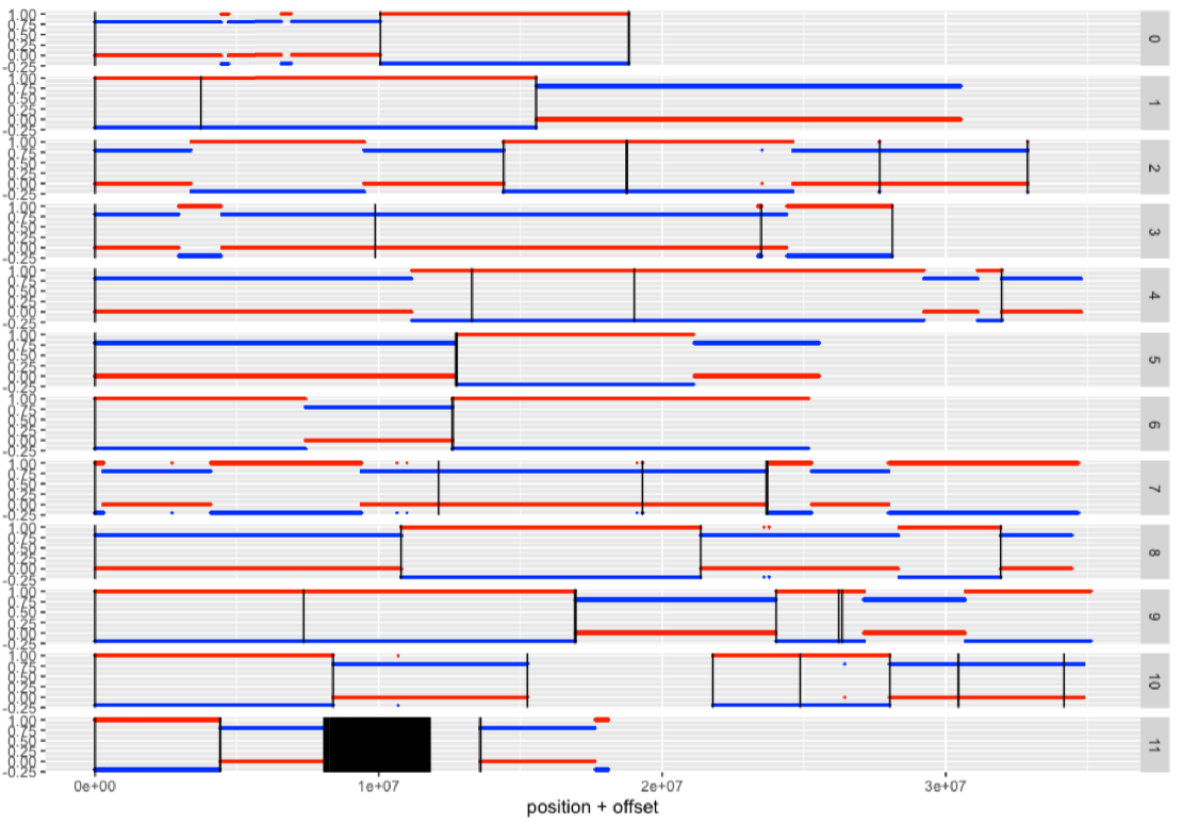
\includegraphics[width=\textwidth]{phasstphase.png}
\floatfoot{\small{Phasst phase shows cleaner phasing than sparse \textit{Bernoulli} mixture model phasing because it skips over any kmer pairs that are not phasing consistent, it only allows discrete phasing instead of a continuous solution, and sex contigs have been detected and skipped. }}
\end{centering}
\end{figure}

\subsection{Haploid / sex contig detection}

\par{
Phasing consistency counts should only be used when the chromosome is diploid (or polyploid if the rules were extended to apply to polyploid genomes). This makes contigs coming from haploid sex chromosomes problematic. It would be desirable to detect these prior to phasing and scaffolding such that they can be treated separately in a more standard fashion of just using Hi-C read linkage as a signal for scaffolding. Kmer counts and kmer pair density are used as signals for diploid contigs. Using a fast kmer package from Gene Myers called FASTK\cite{fastk}, I find all kmers that occur exactly once in the assembly and check their counts in the HiFi data and take the mean for each contig. For kmer pair density, I simply find how many of the kmer pairs occur on each contig and divide by the contig length. Figure \ref{figure:sexcontigs} shows contig kmer counts vs kmer pair density for \textit{Vanessa atalanta} for contigs > 100kb.
}

\begin{figure}[htbp!]
\caption{Haploid / sex contig detection for \textit{Vanessa atalanta}}
\label{figure:sexcontig}
\begin{centering}
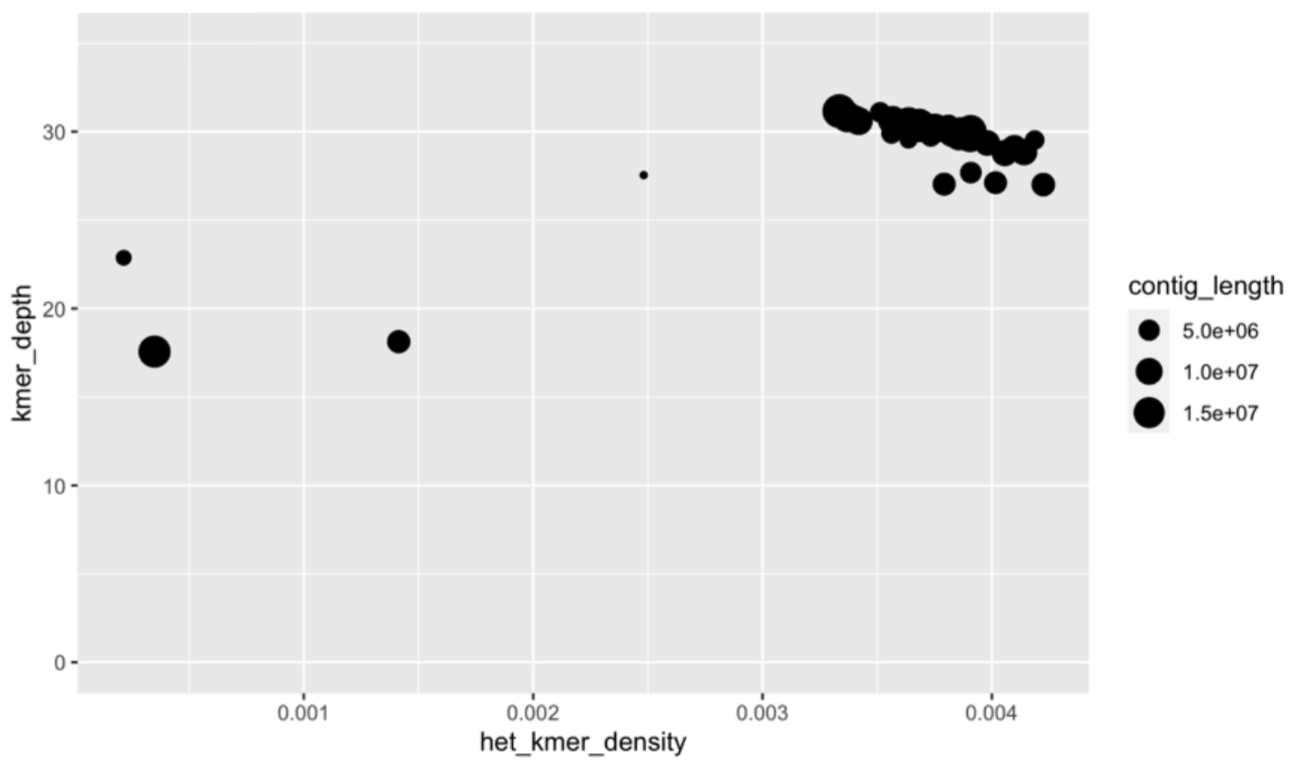
\includegraphics[width=0.65\textwidth]{sexcontig.png}
\floatfoot{\small{Kmer counts are a signal for haploid/sex contigs, but only a weak one because the heterozygosity for this species is so large, much of the sequencing in diploid chromosomes are haploid counts. Kmer pair density is a much better signal for haploid contigs. The three contigs on the left of the graph are sex contigs. The one intermediate contig is just over 100kb and we do not know if it is diploid or not. }}
\end{centering}
\end{figure}

\par{
While haploid sex contig detection works well for this dataset and assembly, it is quite different for different species. This could be due to pseudoautosomal regions, repeat structure, or several other factors. An alternative method would be to use orthologous genes known to be on sex chromosomes in related species for sex contig detection.
}

\subsection{Contig breaking}

\par{
Before scaffolding, one should break any contigs which are likely chimeric misassemblies. This is a common first step in scaffolding\cite{SALSA}\cite{scaffoldingreview}. The Hi-C data is used to break contigs across regions where there are extremely low or no Hi-C links. Both paired kmers as well as a modimized sampling of likely homozygous kmers are used in order to utilize more of the data. A window is sweeped across kmer positions on the contig and count how many Hi-C links cross the midpoint of that window. Both raw counts and phasing consistency counts of kmer pairs across the midpoint of the window are kept separately. Figure \ref{figure:contigbreaking} shows a depiction of this process as well as data on a contig which contains a chimeric misassembly and requires breaking from the \textit{Vanessa atalanta} HiCanu assembly. I show both total links across the midpoint of a 200 kmer pair window as well as the percent phasing consistency across that window. In this case, the total links drops to zero, so of course the phasing consistency also drops to zero, but one can see how phasing consistency for breaking contigs can be a very powerful signal. However, this does require that one has detected the sex contigs and treat them differently. With this, I found the same three breaks in the HiCanu assembly that SALSA does.
}

\begin{figure}[htbp!]
\caption{Contig breaking using Hi-C total linkage and phasing consistency}
\label{figure:contigbreaking}
\begin{centering}
\sidesubfloat[]{
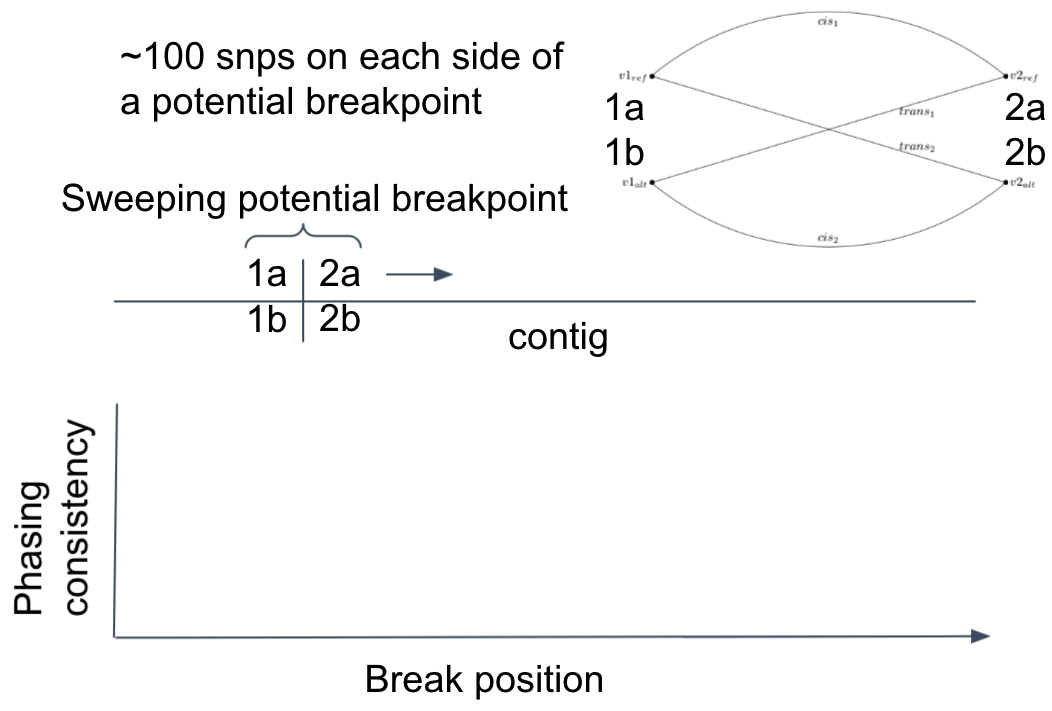
\includegraphics[width=0.75\textwidth]{contigbreaksdiagram.png}
} \\
\sidesubfloat[]{
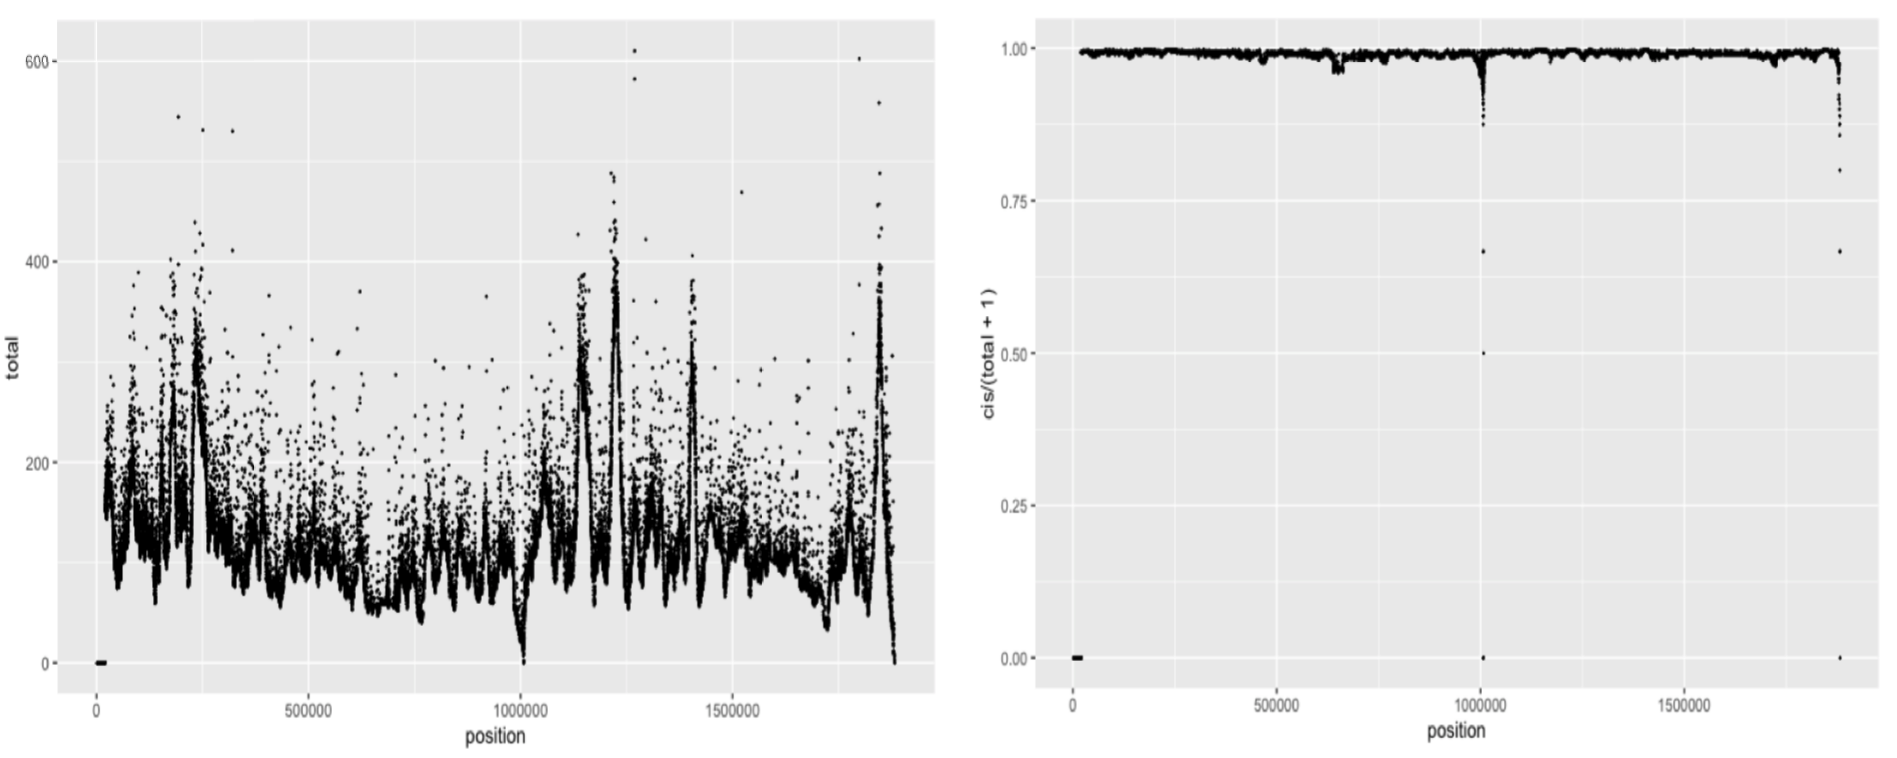
\includegraphics[width=\textwidth]{contigbreaksdata.png}
}
\floatfoot{\small{\textbf{a)} shows the setup for contig breaking. A 200bp window is used and the linkage and phasing consistency are calculated across the midpoint of a sliding window. Below, \textbf{b)} shows the results of this at each position of that sliding window. }}
\end{centering}
\end{figure}



\section{Phasstools: phasing and assembly tools}

\subsection{Phasst scaff: phasing aware assembly scaffolding}

\par{
Now that the paired kmers are phased on each contig, at least for the ones that could be phased, one can now look at the phasing consistency counts of pairs of contigs by looking at Hi-C reads that contain kmer pairs that occurs on two contigs. An example of a phasing consistent match we found has the following counts:  cis1: 10150, cis2: 10278, trans1: 98, trans2: 101. A binomial test is used to compare cis vs trans counts to a random expectation of 0.5 and of course these numbers yield exceedingly low p-values. The counts between non matches are essentially randomly distributed between cis and trans. For the HiCanu assembly of the butterfly \textit{Vanessa atalanta}, the system found the same scaffolding matches that SALSA2 finds.
}

\subsubsection{Chromosome binning}

\par{
Using these matches, a graph is created where nodes are contigs and edges are phasing consistent scaffolding matches. The connected components of this graph are found and these connected components of contigs represent the chromosomes these contigs belong to. 
}

\subsubsection{Order and orientation}

\par{
To order and orient, the heterozygous and homozygous kmers on the ends of each contig (100,000 bases on each contig end, or to the middle of the contig if shorter then 200kb) are used. Counts of how many Hi-C reads link the start and end of each contig to the start and end of each other contig in the chromosome bin are calculated. This number is then normalized by the actual length used (if less than 100,000). The next part, I have not completed, but I will describe the plan and how it differs from what is currently done. Essentially, SALSA takes these normalized link numbers between the ends of each contig that passes its scaffolding thresholds and takes the highest weight link and makes that a new longer scaffold and then the next highest weight until completion. I intend to create a stochastic process in which the edges are chosen with a probability weighted on the normalized linkage value and otherwise proceed as SALSA does. This process will be run many times and the final scaffolding will be selecte that maximizes the total sum of normalized linkage weights. Foe each link, I will be able to report what percentage of the stochastic scaffoldings it was chosen to give a level of confidence to the ordering and orientation.
}

\subsection{Phasst a: phased assembly}

\par{
I applied this method to \textit{Vanessa atalanta}, the Red Admiral butterfly, for which we have $\approx$40x PacBio HiFi data and $\approx$90x 10x Genomics linked read data for the same individual. The heterozygosity is roughly 1.1\%, which is roughly an order of magnitude higher than the average heterozygosity of humans, which is $\approx0.1\%$.
} 

\par{
Our first attempt at phased assembly simply used pairwise phasing consistency of kmer pairs. I created a graph where kmer pairs are nodes and edges exist if the two kmer pairs are phasing consistent. I made an edge between two kmer pairs if the phasing consistency was >90\%, minor edge of the major phasing was >15\%, and there were at least 10 total counts. This creates megabase scale graphs that are linear on a global level. Figure \ref{figure:phasegraph} shows examples of these graphs visualized in Gephi with graph layout force atlas 2\cite{gephi}\cite{forceatlas2}. 
}

\begin{figure}[htbp!]
\caption{Example phasing consistency graph contigs for \textit{Vanessa atalanta}}
\label{figure:phasegraph}
\begin{centering}
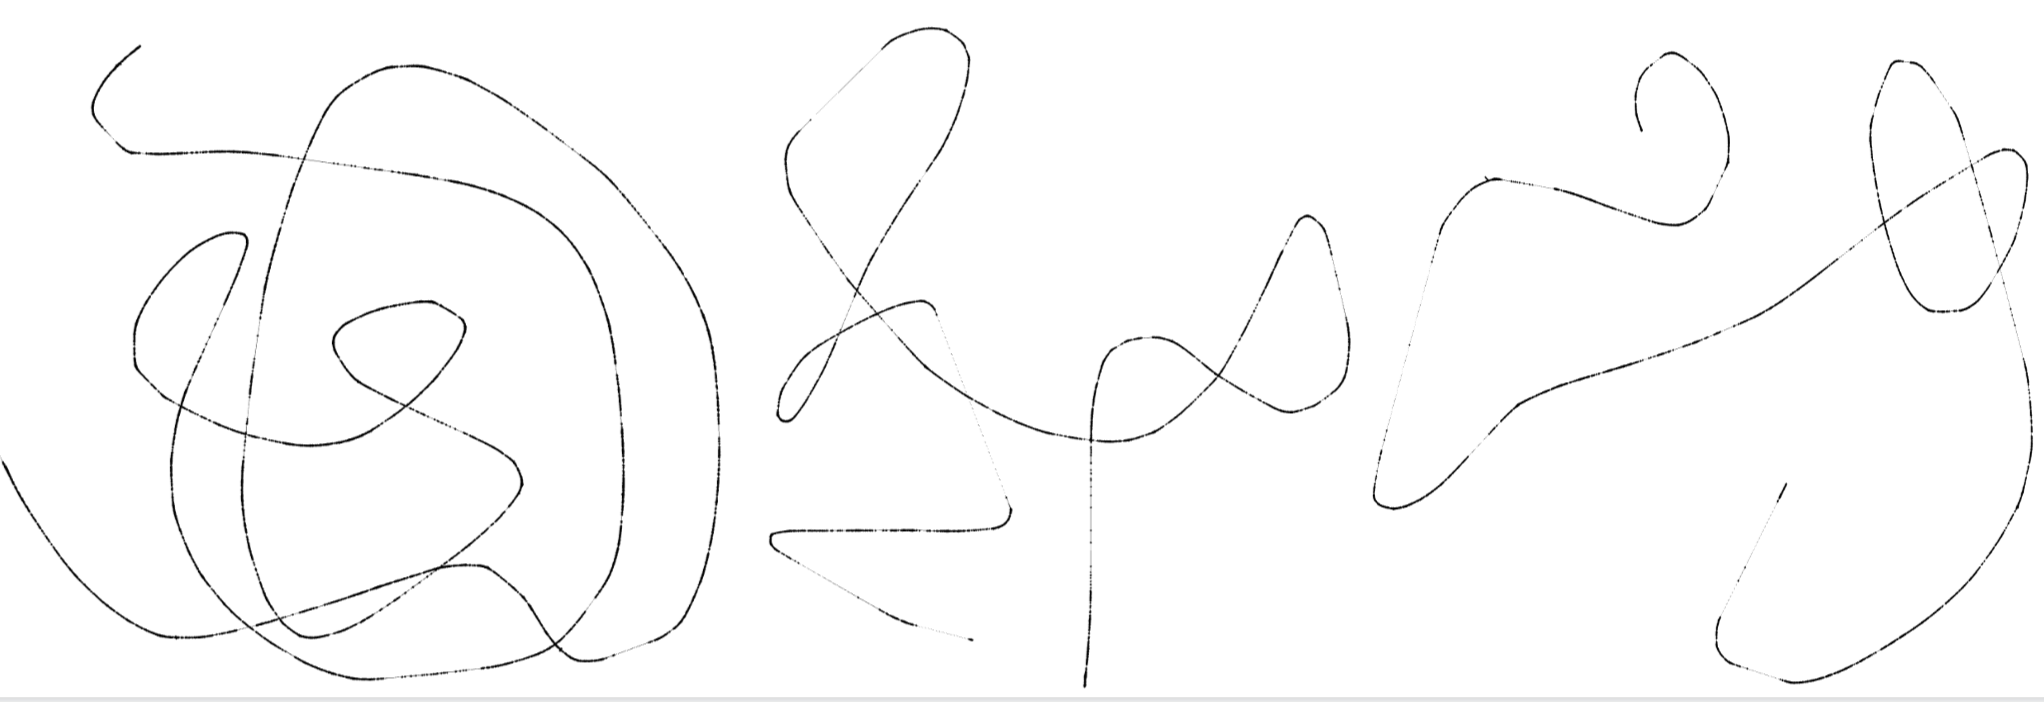
\includegraphics[width=\textwidth]{phasinggraph.png}
\floatfoot{\small{Graph of kmer pairs with edges between them if they are phasing consistent. }}
\end{centering}
\end{figure}

\par{
The idea is to then use these phasing consistency graphs as psuedo contigs from which kmer pairs can be phased, and then bin reads into haplotypes within those contigs and do haploid assembly of those reads. Unfortunately, not all of these graphs were globally linear. This meant that some edges were incorrect. Increasing the stringency of the phasing consistency thresholds did not get rid of all of these spurious connections. If we proceeded with this plan, this could lead to chimeric misassemblies. Figure \ref{figure:misassemblygraph} shows two examples of these misassembly causing connections.
}

\begin{figure}[htbp!]
\caption{Example of errors in phasing consistency graph for \textit{Vanessa atalanta}}
\label{figure:misassemblygraph}
\begin{centering}
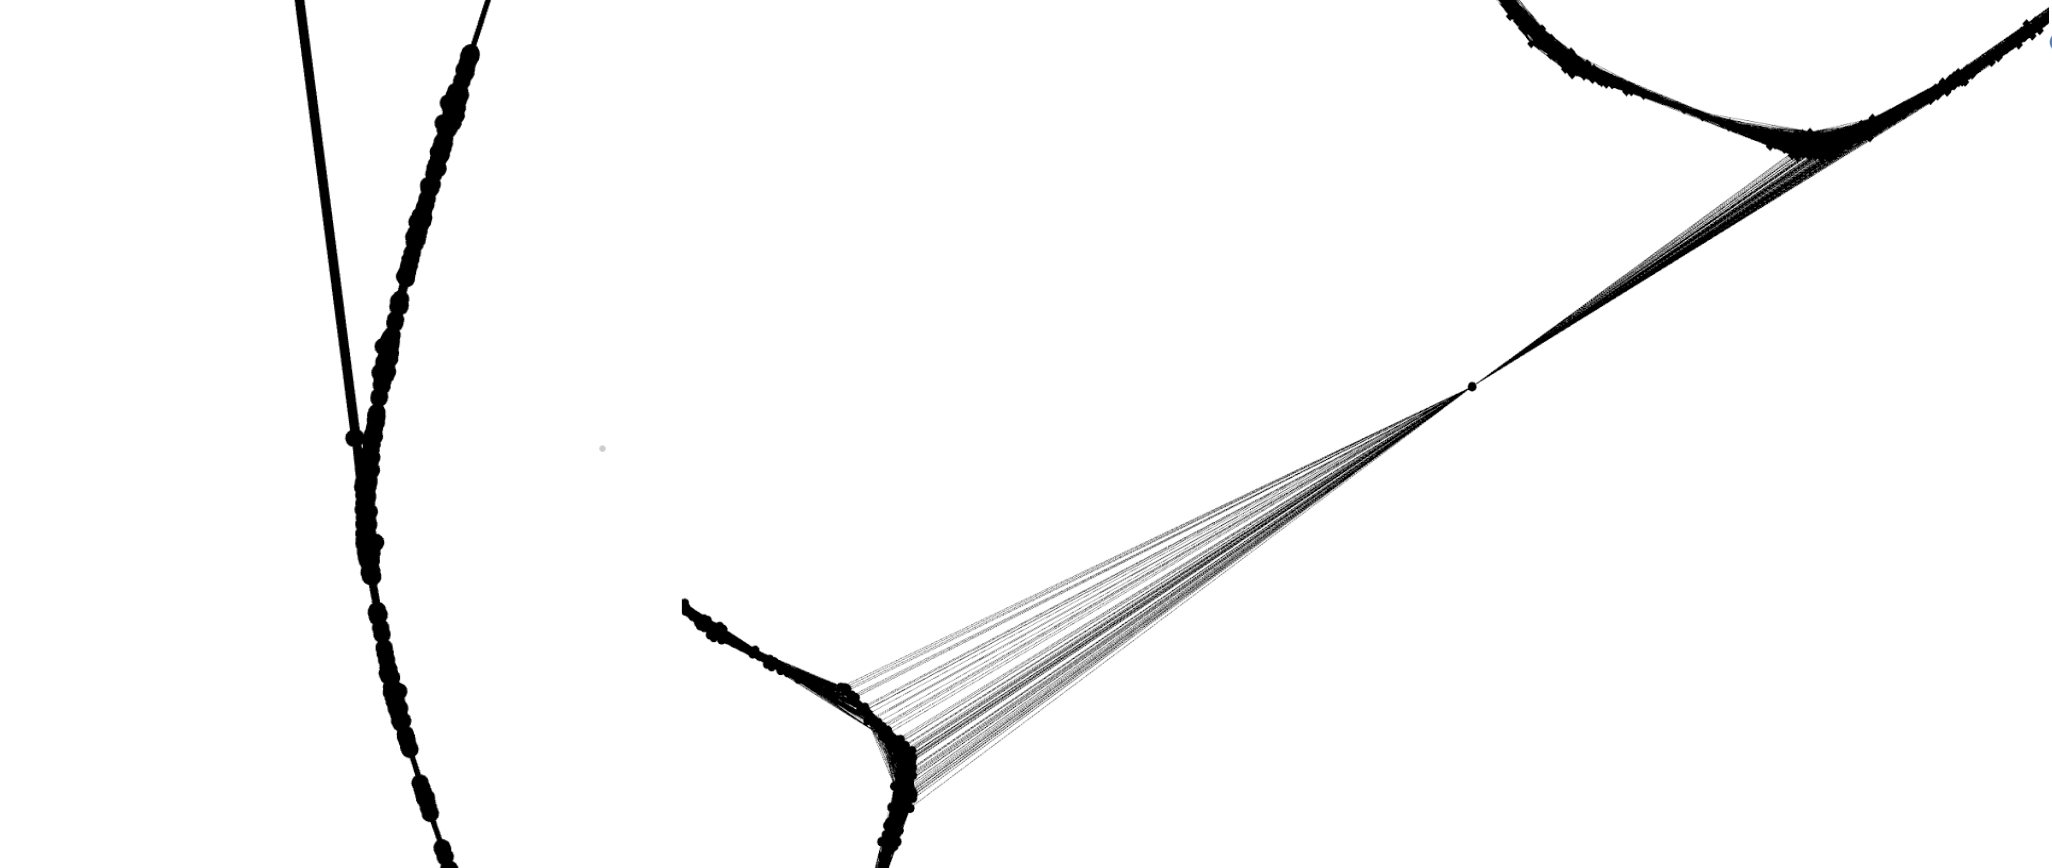
\includegraphics[width=\textwidth]{misassemblyphase.png}
\floatfoot{\small{Errors in misassembly graph. On the left there is an error in which a single kmer pair is phasing consistent with another single kmer pair elsewhere in the genome. This type of error reduces as the phasing consistency thresholds are made more striict, but the resulting graph becomes more and more fractured. On the right, a single kmer pair consistent with many kmer pairs in two locations. This is because this kmer pair is truly heterozygous in both locations in the genome. This error mode does not reduce with further stringency. }}
\end{centering}
\end{figure}

\subsubsection{Phasing consistent heterozygous kmer recruitment}

\par{
To overcome these problems, each new kmer pair should be phasing consistent with multiple prior kmer pairs. To create an ordering of kmers, I begin with a seed kmer pair that has sufficient other kmer pairs it is phasing consistent with on a pairwise basis. Then a graph of kmers is made using the HiFi reads taking into account directionality by also building the graph and the reverse of that graph for the reverse complement of that kmer (see figure \ref{figure:assemblygraph}) adding edge counts if the edge already exists. From the seed kmer, this graph is searched in a breadth first to choose an order in which to assess new kmers in a directional fashion. Then, at each step, the front kmer pair is popped off of the priority queue and assessed for phasing consistency. If the counts they are sufficiently phasing consistent (>90\% cis or trans, minor allele fraction of >15\%, >10 total phasing consistency counts), that kmer pair is added to the growing phase block in the appropriate phase (whether its dominant counts were cis or trans). And then all molecules containing that kmer pair, if not marked as already used, update phasing consistency counts for other kmer pairs and then marked as used. If the kmer pair is not sufficiently phasing consistent, it is marked as used and unphased and the process continues. This proceeds in this manner until the priority queue is empty. To build the phase block in the other direction from the beginning, the process is reseeded at the initial seed and kmer pairs are added to the priority queue in the opposite direction, keeping track of phasing consistency counts and building the phase block in the other direction until finished. For this step, both HiFi and linked reads are used, both of which have a very low error/cross haplotype signal. Only the HiFi data is used to build the kmer recruitment graph as the linked reads don't have direction across different reads within the same barcode.
}

\begin{figure}[htbp!]
\caption{Kmer recruitment graph}
\label{figure:assemblygraph}
\begin{centering}
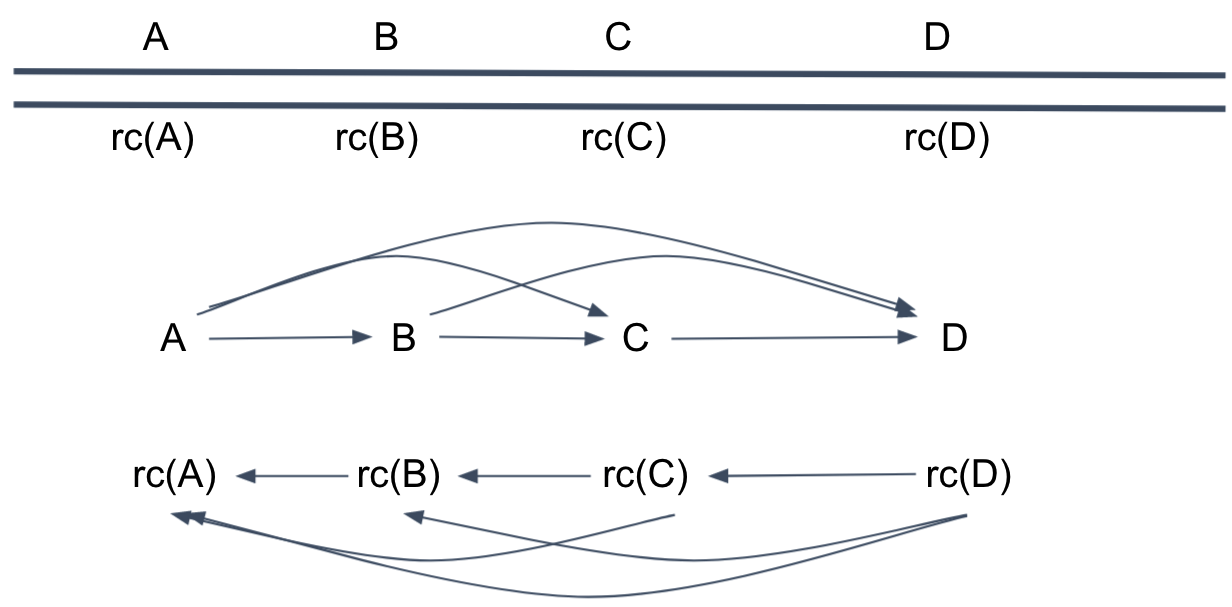
\includegraphics[width=0.8\textwidth]{assemblygraph.png}
\floatfoot{\small{Kmer recruitment graph from HiFi reads. }}
\end{centering}
\end{figure}

\subsubsection{Contig and haplotype read binning}

\par{
Once this kmer pair phased assembly is done, it is used to assign HiFi reads to contigs and haplotypes within contigs. Each read's kmer content is inspected and kmer counts for each contig/haplotype are calculated. Usually, the match is unanimous, but in the case of conflict, the read is assigned if it favors one contig haplotype by three or more kmers. 
}

\subsubsection{Haploid chromosome assembly}

\par{
Now that reads are binned to contigs and haplotypes, the next step is haploid assembly. The miniasm assembler is used with parameters suited to HiFi data as opposed to the defaults which were for the more noisy CLR data\cite{miniasm}. This may result in a single contig per assembly phase block or multiple contigs. }

\par{ To validate, the contigs from these assemblies are mapped to the HiCanu assembly. The contiguity of this assembly is less than HiCanu, with an N50 of $\approx$900kb. And there are sometimes interesting heterozygous differences between the two haplotype assemblies. In figure \ref{figure:assemblyplot} the haplotype assemblies of one assembly phase block aligned to the HiCanu reference is shown. In one haplotype, the full phase block was assembled as a single contig. The other haplotype assembled into three contigs. The haplotype read sets aligned to the HiCanu assembly were inspected in IGV (not shown) as well as the bandage plot for the GFA from the miniasm assembly of that haplotype, and there is evidence for a 35kb duplication flanking a 23kb unique sequence\cite{bandage}. This duplication does not appear to exist on the other haplotype.
}

\begin{figure}[htbp!]
\caption{Example of heterozygous structural variation.}
\label{figure:assemblyplot}
\begin{centering}
\sidesubfloat[]{
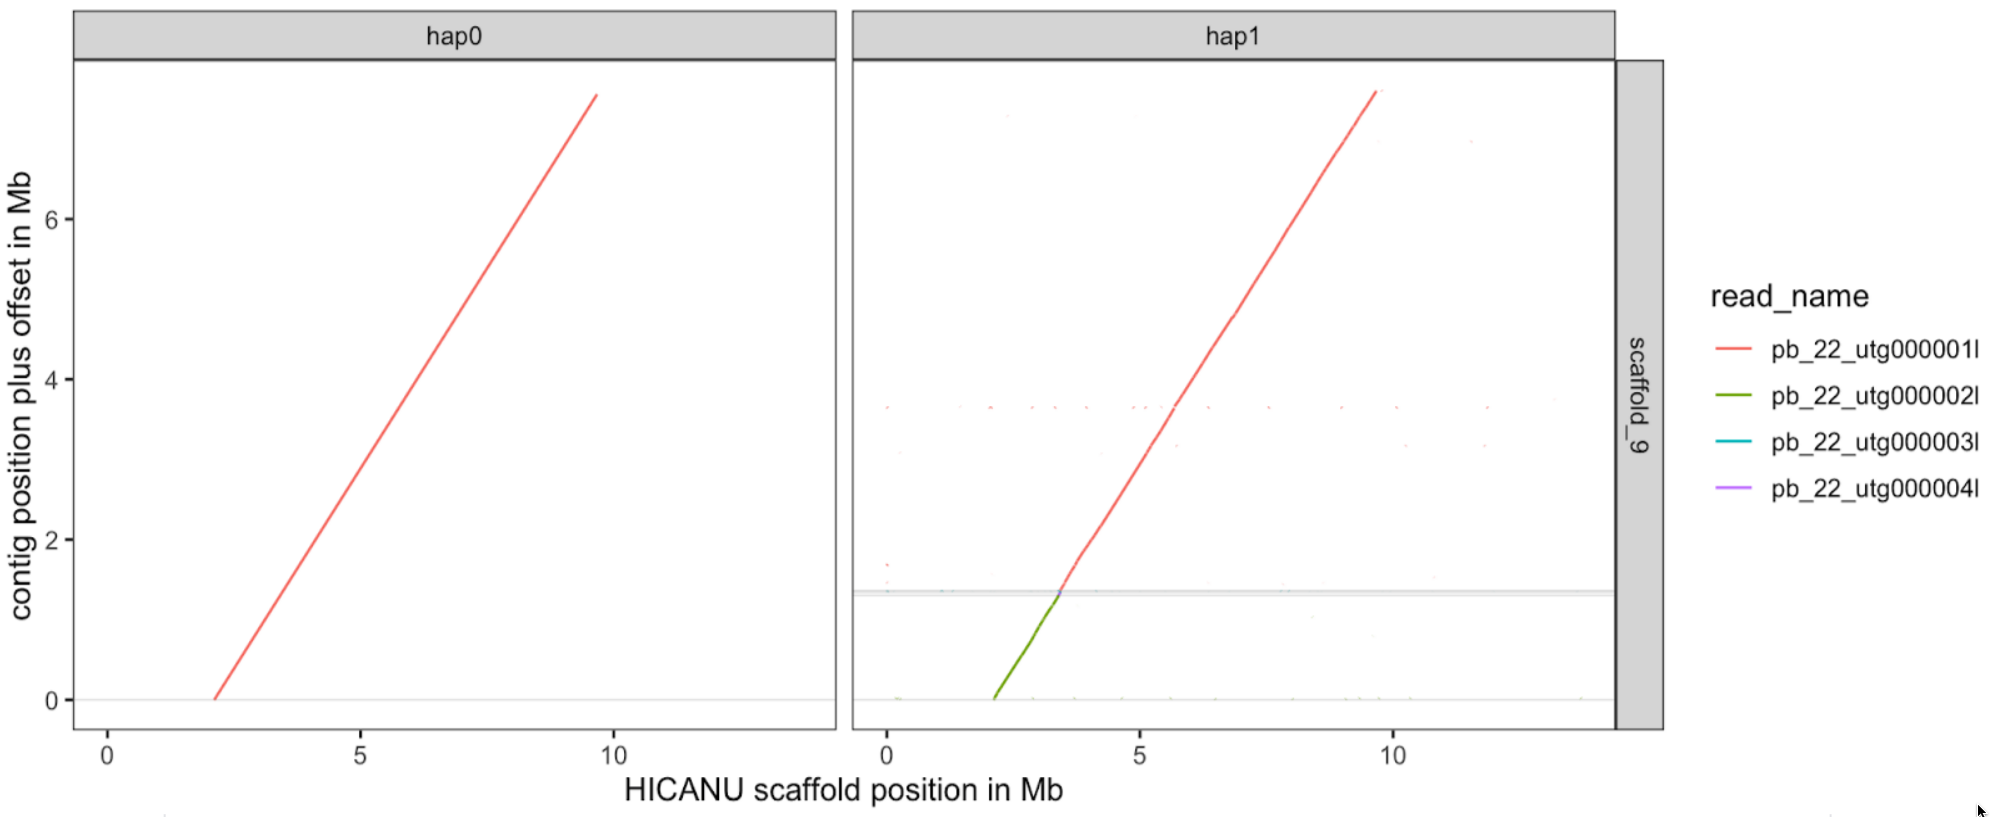
\includegraphics[width=0.75\textwidth]{haplotypeassembly.png}
} \\
\sidesubfloat[]{
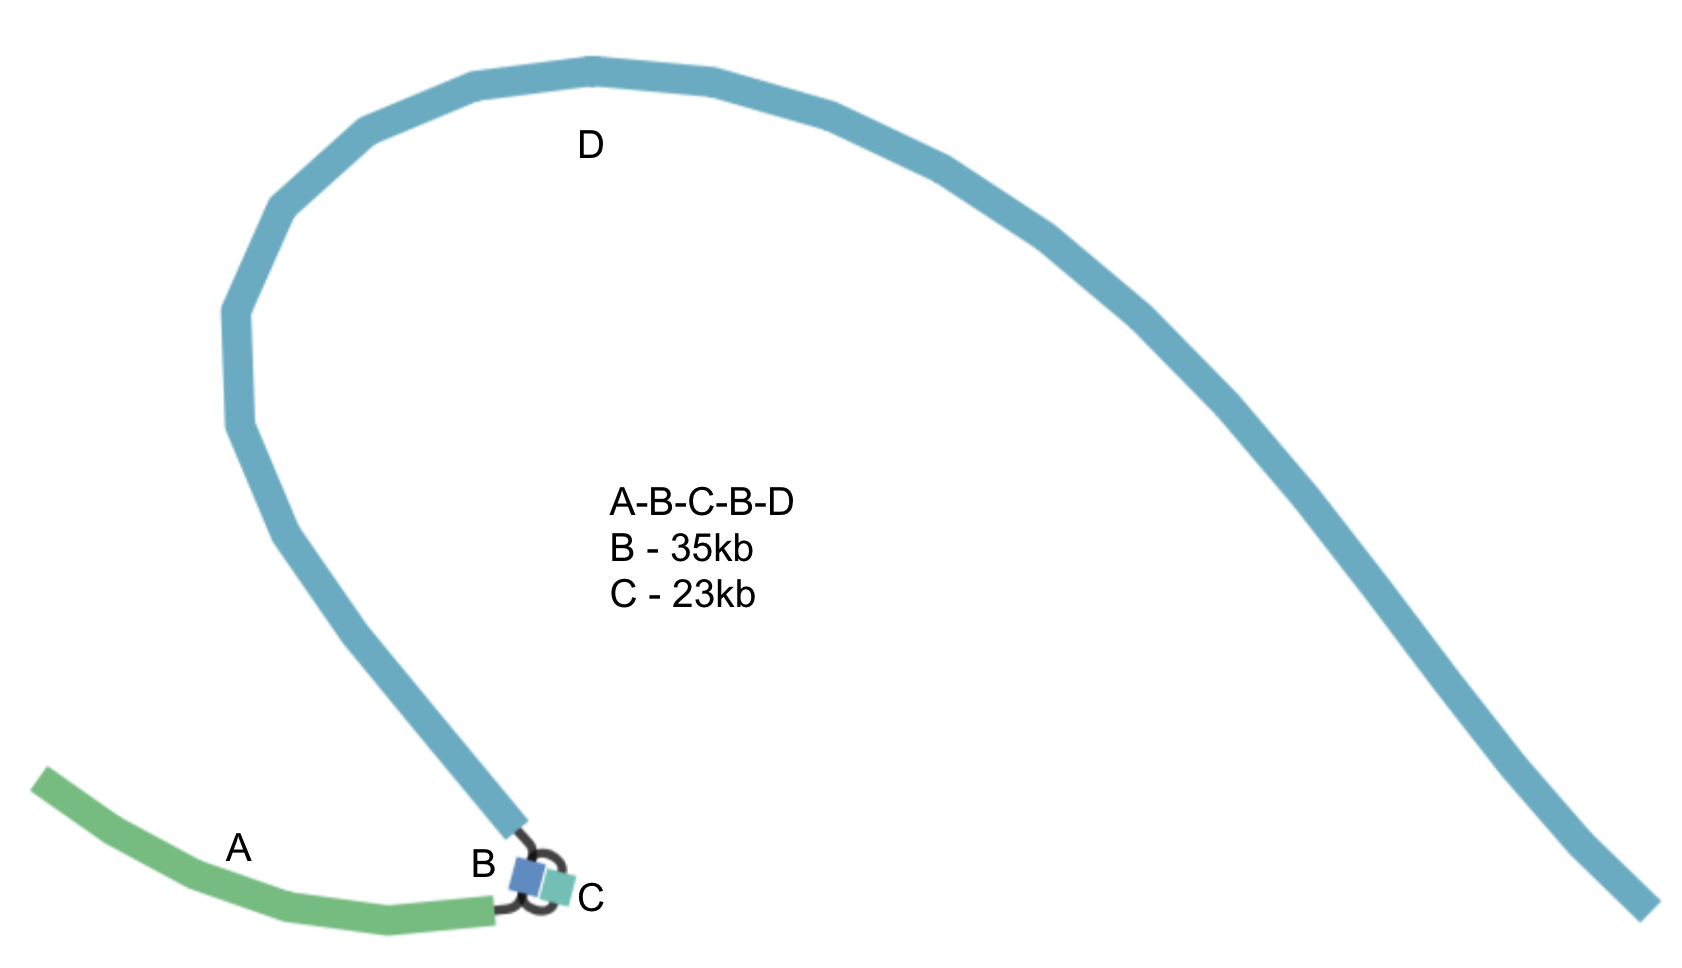
\includegraphics[width=0.75\textwidth]{bandage.png}
}
\end{centering}
\floatfoot{\small{\textbf{a)} alignment plots of haplotype contigs vs HiCanu assembly shows one haplotype not assembling into a single contig because \textbf{b)} one haplotype has a $\approx$35kb repeat that is not present in the other haplotype. HiCanu retained the haplotype that was most contiguously assembled.}}
\end{figure}

\subsubsection{Assembly contig coverage vs HiCanu assembly}

\par{
One of the haplotype assemblies from each assembly phase block was aligned to the HiCanu assembly to inspect the overall contig coverage of our assembly\ref{figure:contigcoverage}. The first thing one notices is that there are three HiCanu contigs with very little assembly coverage. These are the haploid sex contigs which do not get assembled by our method as it currently stands. The more complex contig on the lower right sex contig is rich in repeat sequence and our system has assembled some of it. The other notable discrepancy between these assemblies is the zero contig coverage areas on the ends of two contigs in rows six and seven. The HiFi read alignments to the HiCanu assembly were inspected and there is no support for this connection. It is unclear where that sequence originated from. Potentially it is truly haploid sequence which got chimerically joined with an otherwise autosomal contig.
}

\begin{figure}[htbp!]
\caption{Assembly contig coverage}
\label{figure:contigcoverage}
\begin{centering}
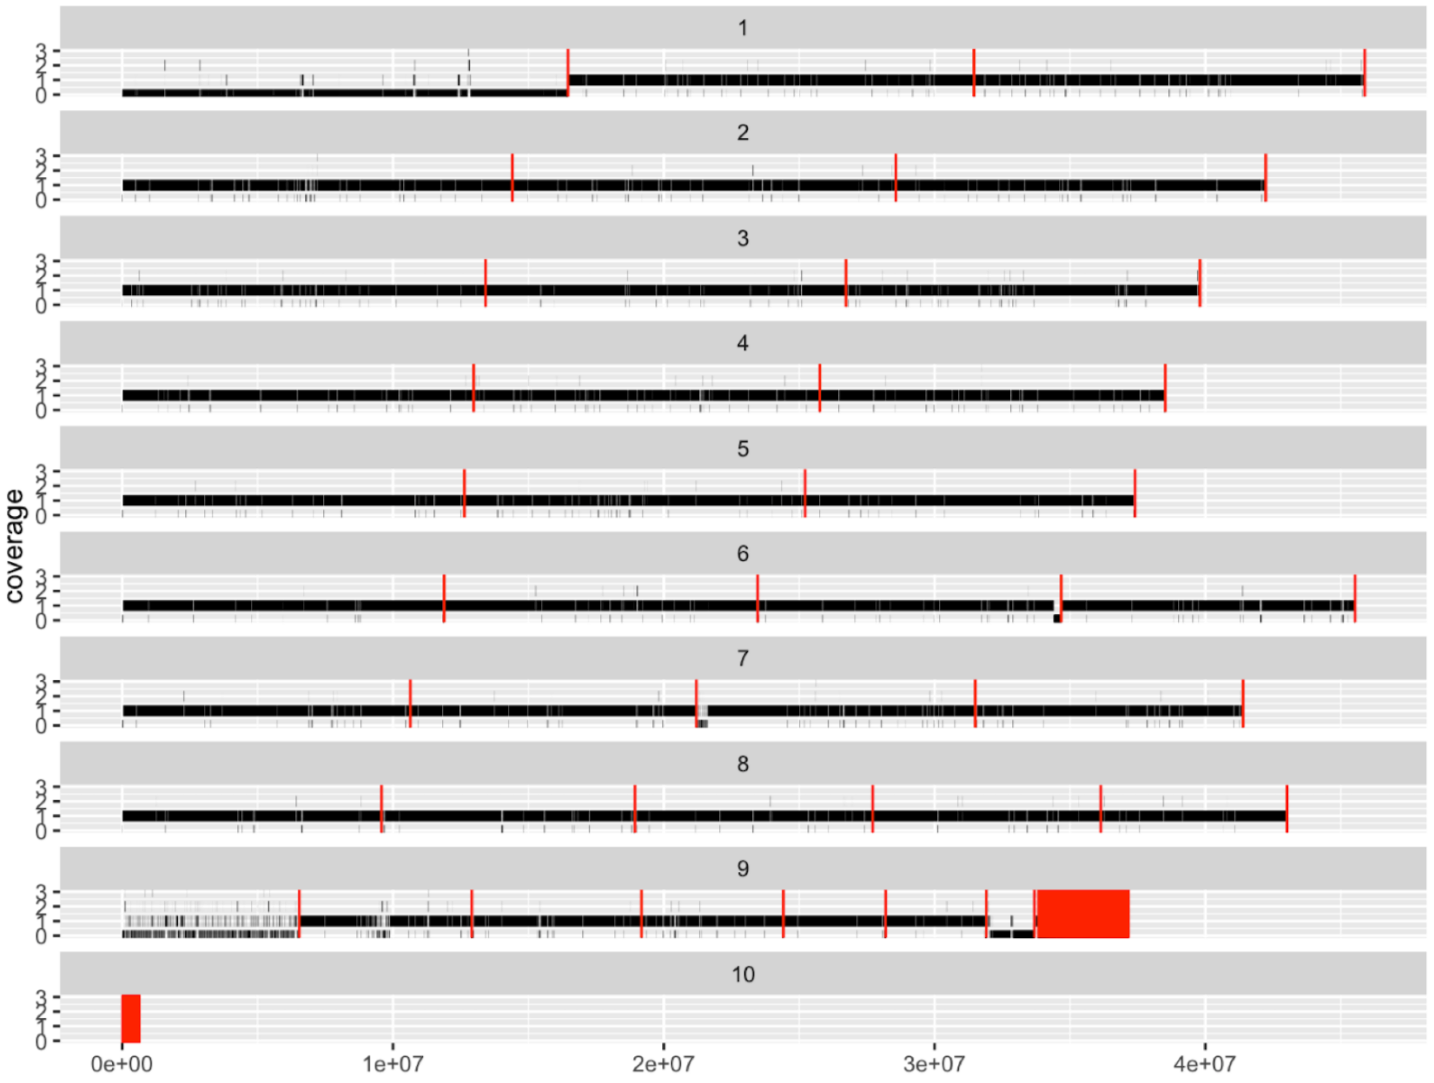
\includegraphics[width=\textwidth]{assemblycontigcoverage.png}
\floatfoot{\small{Contig coverage of one haplotype of the phased assembly aligned to the HiCanu assembly. The haploid sex contigs have not been assembled. The drops in coverage on two chromosomes in rows six and seven have been determined to be misassemblies in the HiCanu assembly. }}
\end{centering}
\end{figure}



\section{Discussion}

\par{
Due to recent advances in long read and long range genetic information technologies, our ability to assemble high quality genomes has increased greatly. But some issues still exist around high heterozygosity and small organisms. With the advent of the Earth Biogenome project and the Darwin Tree of Life project, there is a need for new assembly and scaffolding methods that are robust to these issues and work on a wide range of organisms. While there are a number of phased assembly methods currently available, I take the approach of treating phasing consistency as a first class signal for physical linkage and make it just as important as sequence similarity in the assembly and scaffolding processes.
} 

\par{
I demonstrated a new phasing aware scaffolding method and compared it to the most commonly used existing scaffolder. It is clear that phasing consistency is a powerful tool in determining if contigs should be scaffolded together or not. There is a dramatic difference between the phasing consistency counts of contigs from the same chromosome and different chromosomes using Hi-C reads.
} 

\par{
I also described a novel algorithm for \textit{de novo} haplotype phasing even without assembling. This algorithm is also capable of scaling to polyploid genomes efficiently by adding more haplotype cluster centers. It is also robust to receiving as input sites that are not actually heterozygous and is capable of correcting the genotypes of those sites. This algorithm is of general use even outside of the context of phasing aware scaffolding. I believe this will be of particular use for plant genome research as many crops are polyploid. When expanded with either a growing window approach or deterministic annealing, I believe that the local optima problems from regionality of many data types will be solved.
} 

\par{
Finally, I presented a method for phased assembly by using heterozygous kmer pairs and their phasing consistency as a signal of physical linkage. I then use this to bin HiFi reads into haploid bins which can be assembled separately. By phasing prior to assembly, the errors and bias caused by the ambiguity between heterozygosity and paralogous sequences are removed. Furthermore, I generate a complete set of paired haplotype sequences, linked by confirmed single-copy kmer-pairs, in the process identifying large scale structural variation.  Although N50 numbers are shorter than from some modern assemblers, I believe the linked haplotype output of our method is the correct goal for diploid assembly. The same approach could in principle be applied to higher ploidy genomes.
}







